% !TeX root = ../../Book3.tex
% 纲要标题：## 第18章　调和映射的变分、正则性与集中
% 纲要位置：几何学计划纲要.md，第 2818 行。
% 正文状态：初稿；尚未正式审核。

% 纲要内容开始
% 
% > 本章目标与证明范围：把光滑临界方程、极小映射、平稳映射和一般弱解分开。完整完成所选小能量正则性模块；热流在抛物工具之后处理，避免局部椭圆正则性与长期存在混同。
% 
% 纲要内容结束

\chapter{调和映射的变分、正则性与集中}
\label{g3:ch:18}
\BookChapterNumber{g3:ch:18}

\begin{chapterabstract}
	调和映射把测地线的能量驻值问题推广到高维源流形。本章从拉回联络推导张力场、第一变分及含目标曲率的第二变分，再用等距嵌入建立流形值 Sobolev 映射的弱框架，区分能量极小、内变分平稳与弱调和方程。在二维圆盘上，从 Bochner 不等式、均值估计与选点论证完整证明光滑调和映射的小能量梯度估计，继而得到高阶内估计，以及闭曲面源上有限集中集之外的光滑紧性与非恒定重缩放极限。曲面上的共形不变性将这些分析与 Hopf 微分、极小曲面联系起来；显式球面映射展示能量集中和弱极限中的度数丢失。二维一般弱解及高维部分正则性采用准确列明假设的外部定理。
\end{chapterabstract}

\begin{learninggoals}
	\begin{itemize}
		\item 构造沿映射的协变导数，推导能量的一阶与二阶变分，并核对曲率项的符号。
		\item 用等距嵌入定义 \(H^1\) 映射，证明定义和内在能量不依赖所选嵌入。
		\item 分清弱调和、平稳与极小三类条件，推导应力张量和内变分单调性公式。
		\item 完成二维光滑解的小能量估计，并说明其尺度、阈值及背景几何依赖。
		\item 从局部估计得到光滑紧性，定位可能的集中点并构造重缩放极限。
		\item 计算 Hopf 微分、共形调和浸入的平均曲率及球面气泡的能量分布。
	\end{itemize}
\end{learninggoals}

把一段曲线的两个端点固定，能量的临界方程是测地线方程。若源换成一块平面区域，映射可以沿两个独立方向变化，临界方程便对这两个方向的协变二阶导数求和。最简单的目标是实直线：此时能量为 \(\frac12\int|\mathrm du|^2\)，临界方程正是标量 Laplace 方程。目标弯曲以后，二阶导数需要投回目标切空间，方程中随之出现梯度的二次项。

\ProseParagraphBreak

这个二次项使有限能量成为一个自然却仍不足以控制逐点行为的条件。将平面圆盘中的映射放大为 \(v(y)=u(a+ry)\)，梯度平方带来 \(r^2\)，面积变换带来 \(r^{-2}\)，两者恰好相消。一份固定的能量因此可能进入越来越小的区域，而总能量保持有界。要恢复紧性，就须证明：局部能量低于某个统一阈值时，梯度和更高阶导数都能受控。超过这一阈值的区域则需要单独观察，重缩放会显露原尺度下看不见的映射。

\ProseParagraphBreak

本章先建立变分公式与弱极限的语言，再完成上述小能量证明。最后的球面模型将给出确切数值：一列度数为一、能量恒为 \(4\pi\) 的光滑调和映射，可以弱收敛到常值映射，全部能量同时集中于一点。固定迹的直接法、固定同伦类的极小化，以及光滑临界点族的紧性，因而具有不同的证明任务。

\ProseParagraphBreak

几何准备是\chapref{g3:ch:03}的曲率约定、\chapref{g3:ch:04}的第二基本形式和管状邻域，以及\chapref{g3:ch:06}的曲线变分。分析准备是\chapref{g3:ch:11}的 Sobolev 链式法则、紧嵌入与迹，以及\chapref{g3:ch:12}、\chapref{g3:ch:14}的内域估计和标量边值问题。曲面部分在本章证明等温坐标的存在，并就近恢复复双线性配对与弱共形的含义；所需的单变量全纯函数结论可查第四卷第1.1节，球面的度数积分公式可查第二卷第16.1.2小节。弱映射所用的 Nash 等距嵌入和\subsecref{g3:subsec:1803:06}的三项弱正则性定理，均在调用处标明正式文献及准确范围。

% !TeX root = ../../Book3.tex
% 纲要标题：### 18.1 能量与几何变分
% 纲要位置：几何学计划纲要.md，第 2822 行。
% 正文状态：初稿；尚未正式审核。

% 纲要内容开始
% 
% * 拉回丛上的协变微分
% * 张力场和第一变分
% * 第二变分及目标曲率
% * 测地线作为一维原型
% 
% 纲要内容结束

\section{能量与几何变分}
\label{g3:sec:1801}

曲线能量把速度的平方沿参数区间积分。对于映射 \(u:M\to N\)，每个源方向都有一个像速度，因而自然把这些速度的平方相加，再在 \(M\) 上积分。临界方程要求各方向的协变加速度之和为零；单个方向的加速度不必为零。为了比较邻近映射，还须把不同点处的目标切向量放在同一个沿映射的向量丛中。本节将\chapref{g3:ch:06}的曲线变分计算推广到这个情形。

\ProseParagraphBreak

变分公式的经典论述可参照\cite[第2节，第115--117页；第6.C节，第135--136页]{EellsSampson1964HarmonicMaps}；以下按本卷的非负 Laplace 与曲率约定逐项推导。

\subsection{拉回丛上的协变微分}
\label{g3:subsec:1801:01}
设 \((M^m,g)\)、\((N^n,h)\) 为光滑黎曼流形，\(m,n\ge1\)，目标 \(N\) 无边界，源 \(M\) 可有光滑边界。除特别说明外，映射及各场均光滑到边界。映射 \(u:M\to N\) 不必是浸入：它可以把一个开集压成一点，也可以在不同源点取同一目标值。沿 \(u\) 的向量场在每个 \(x\) 处属于 \(\mathrm T_{u(x)}N\)，这些空间组成\term[lahui qiecong]{拉回切丛}[pullback tangent bundle]
\[
	u^*\mathrm TN=\{(x,v):x\in M,\ v\in\mathrm T_{u(x)}N\}\longrightarrow M.
\]
它的两个自然投影组成交换图
\[
	\begin{tikzcd}
		u^*\mathrm TN \arrow[r,"\widetilde u"] \arrow[d] & \mathrm TN \arrow[d,"\pi_N"]\\
		M \arrow[r,"u"] & N.
	\end{tikzcd}
\]
这里 \(\widetilde u(x,v)=v\)。图中左侧的纤维保留源点 \(x\)，即使两个源点有相同像，也仍是两个不同纤维。在目标坐标 \((y^\alpha)\) 中，截面写成 \(V=V^\alpha\partial_{y^\alpha}|_u\)。这里 \(V^\alpha\) 是源上的函数，\(V\) 则是沿映射的场，不是定义在整个目标上的向量场。

\ProseParagraphBreak

目标的 Levi-Civita 联络诱导 \(u^*\mathrm TN\) 上的联络，记为 \(D\) 或 \(\nabla^u\)。其坐标表达为
\begin{equation}\label{g3:eq:pullback-connection-coordinates}
	(D_XV)^\alpha
	=X(V^\alpha)+\Gamma^\alpha_{\beta\gamma}(u)\,X(u^\beta)V^\gamma.
\end{equation}
这个定义与坐标无关。事实上，在目标局部标架 \((E_a)\) 中写 \(V=v^aE_a\circ u\)，可写成
\[
	D_XV=X(v^a)E_a\circ u+v^a\nabla^N_{\mathrm du(X)}E_a.
\]
若 \(E'_a=E_bQ^b_a\)，对 \(Q(u)\) 求导所得 \(X(Q\circ u)=\mathrm dQ(\mathrm du(X))\) 项，正与目标联络的换架项相抵消，得到同一个截面。因此局部定义粘合。目标联络的度量相容性还给出
\[
	X\langle V,W\rangle_h=\langle D_XV,W\rangle_h+\langle V,D_XW\rangle_h.
\]
这说明可以像对普通向量场一样求导内积，而不必先把 \(V,W\) 延拓到 \(N\)。

\ProseParagraphBreak

微分 \(\mathrm du\) 是 \(\mathrm T^*M\otimes u^*\mathrm TN\) 的截面。将源与目标联络结合，定义其协变微分
\begin{equation}\label{g3:eq:map-second-covariant-differential}
	B_u(X,Y)=(\nabla\mathrm du)(X,Y)
	\coloneqq D_X(\mathrm du(Y))-\mathrm du(\nabla^M_XY).
\end{equation}
减去第二项，是为了扣除源方向 \(Y\) 本身的变化。联络的 Leibniz 法则说明这个差对 \(X,Y\) 都是函数线性的，因此是一个真正的二阶协变张量，而非依赖延拓的二次求导。

\begin{proposition}\label{g3:prop:map-covariant-identities}
	设 \((M^m,g)\)、\((N^n,h)\) 为光滑黎曼流形，\(m,n\ge1\)，\(M\) 允许光滑边界，\(N\) 无边界，\(u:M\to N\) 光滑。对拉回联络 \(D\)、光滑源向量场 \(X,Y\) 和沿 \(u\) 的光滑场 \(V\)，记 \(B_u(X,Y)=D_X(\mathrm du(Y))-\mathrm du(\nabla^M_XY)\)，\(R^N\) 采用 \(R(X,Y)=[\nabla_X,\nabla_Y]-\nabla_{[X,Y]}\)。有
	\begin{equation}\label{g3:eq:map-pullback-identities}
		B_u(X,Y)=B_u(Y,X),\qquad
		[D_X,D_Y]V-D_{[X,Y]}V=R^N(\mathrm du(X),\mathrm du(Y))V.
	\end{equation}
	若 \(U:I\times M\to N\) 为光滑映射，\(I\subset\mathbb R\) 为开区间，\(X\) 按与参数 \(t\) 无关的方式提升到乘积上，记 \(V=\partial_tU\)，则
	\begin{equation}\label{g3:eq:map-variation-commutation}
		D_t(\mathrm dU(X))=D_XV,\qquad
		[D_t,D_X]Z=R^N(V,\mathrm dU(X))Z
	\end{equation}
	对每个沿 \(U\) 的光滑场 \(Z\) 成立。
\end{proposition}
\begin{proof}
	在源坐标 \((x^i)\) 中，由式\eqref{g3:eq:pullback-connection-coordinates}得到
	\[
		(B_u)^\alpha_{ij}
		=\partial_i\partial_j u^\alpha
		-\Gamma^k_{ij}(g)\partial_k u^\alpha
		+\Gamma^\alpha_{\beta\gamma}(h)(u)\partial_i u^\beta\partial_j u^\gamma.
	\]
	两个 Levi-Civita 联络都无挠，故各 Christoffel 符号对下面两指标对称；右边因此在 \(i,j\) 之间对称。

	为了计算曲率，在目标标架中记联络矩阵为 \(\omega\)。拉回联络的矩阵就是 \(u^*\omega\)，所以它的曲率矩阵为
	\[
		\mathrm d(u^*\omega)+u^*\omega\wedge u^*\omega
		=u^*(\mathrm d\omega+\omega\wedge\omega).
	\]
	两边作用于 \((X,Y)\) 和截面 \(V\)，正是式\eqref{g3:eq:map-pullback-identities}的第二式。这也可以由坐标式展开两次导数得到：含二阶 \(V\) 导数和一阶 \(V\) 导数的项抵消，留下目标曲率作用于两个像方向。

	最后把同一计算用于 \(U:I\times M\to N\)。因为 \([\partial_t,X]=0\)，无挠性给出 \(D_t\mathrm dU(X)=D_X\mathrm dU(\partial_t)\)，拉回曲率公式给出第二式。这里不要求 \(U\) 是浸入，与\cref{g3:prop:variation-commutation}中的二参数曲线计算一致。
\end{proof}

能量需要在所有源方向上取平方和。若 \((e_i)_{i=1}^m\) 是源的局部正交单位标架，则
\[
	|\mathrm du|^2=\sum_{i=1}^m|\mathrm du(e_i)|_h^2
	=g^{ij}h_{\alpha\beta}(u)\partial_i u^\alpha\partial_j u^\beta.
\]
这是两侧度量在张量丛 \(\mathrm T^*M\otimes u^*\mathrm TN\) 上诱导的范数平方，正交换架不改变这个和。
\begin{definition}\label{g3:def:map-energy}
	设 \(u:(M^m,g)\to(N^n,h)\) 为光滑黎曼流形之间的光滑映射，\(m,n\ge1\)，\(N\) 无边界，\(M\) 允许光滑边界。定义其\term[nengliang midu]{能量密度}[energy density]及在可测区域 \(A\subset M\) 上的能量为
	\begin{equation}\label{g3:eq:map-energy}
		e(u)=\frac12|\mathrm du|^2,\qquad
		E(u;A)=\int_A e(u)\,\mu_g.
	\end{equation}
	积分允许为无穷；\(E(u;M)\) 简记为 \(E(u)\)。当 \(M\) 紧时，光滑映射的能量有限。
\end{definition}
\symidx{\(E(u;A)\)：映射在区域 \(A\) 上的能量}
\symidx{\(e(u)\)：映射的能量密度}
积分使用体积密度，所以源和目标都无须可定向。常映射的微分为零，能量也为零；反之，连通源上的光滑映射若能量为零，则微分处处为零，沿道路积分可知它是常映射。源不连通时，只能得到各连通分支上分别为常值。

\subsection{张力场和第一变分}
\label{g3:subsec:1801:02}
二阶张量 \(B_u\) 同时记录许多源方向。能量对源方向作了求和，其变分方程相应地取这个张量的迹。
\begin{definition}\label{g3:def:tension-harmonic-map}
	设 \(u:(M^m,g)\to(N^n,h)\) 为光滑映射，\(m,n\ge1\)，目标无边界，源允许光滑边界。记 \(D\) 为由目标 Levi-Civita 联络拉回的联络，\(e_i\) 为源的局部正交标架。其\term[zhangli chang]{张力场}[tension field]为沿 \(u\) 的场
	\begin{equation}\label{g3:eq:tension-definition}
		\tau(u)=\operatorname{tr}_g\nabla\mathrm du
		=\sum_{i=1}^m\bigl(D_{e_i}\mathrm du(e_i)-\mathrm du(\nabla^M_{e_i}e_i)\bigr).
	\end{equation}
	若 \(\tau(u)=0\) 于源的内部，则称 \(u\) 为\term[tiaohe yingshe]{调和映射}[harmonic map]。
\end{definition}
\symidx{\(\tau(u)\)：映射的张力场}
张量取迹使定义与源标架无关。局部坐标表达为
\begin{equation}\label{g3:eq:tension-coordinates}
	\begin{aligned}
		\tau(u)^\alpha
		&=g^{ij}\left(\partial_i\partial_j u^\alpha
		-\Gamma^k_{ij}(g)\partial_k u^\alpha
		+\Gamma^\alpha_{\beta\gamma}(h)(u)\partial_i u^\beta\partial_j u^\gamma\right)\\
		&=-\Delta_g u^\alpha
		+g^{ij}\Gamma^\alpha_{\beta\gamma}(h)(u)\partial_i u^\beta\partial_j u^\gamma.
	\end{aligned}
\end{equation}
第二行中的 \(u^\alpha\) 是当前目标坐标中的实函数；它只在该坐标适用的源区域上有意义。目标为 Euclid 空间时，Christoffel 项为零，所以 \(\tau(u)=-\Delta_g u\)。这核对了本书非负 Laplace 算子与张力场之间的负号。

\ProseParagraphBreak

对紧源上的光滑映射 \(u\)，取光滑变分 \(U:(-\varepsilon,\varepsilon)\times M\to N\)，令 \(u_t=U(t,\cdot)\)、\(u_0=u\)、\(V=\partial_tU|_0\)。任意光滑截面 \(V\in\Gamma(u^*\mathrm TN)\) 都可由
\[
	u_t(x)=\exp_{u(x)}(tV(x))
\]
实现。指数映射在零截面附近光滑，源紧且 \(V\) 光滑，因而有共同的充分小参数区间；这个构造不要求目标完备。若 \(V|_{\partial M}=0\)，所得变分逐点固定边界。这里沿用式\eqref{g3:eq:exponential-field-variation}的构造，只把紧参数区间换成了紧源流形。

\begin{theorem}\label{g3:thm:harmonic-map-first-variation}
	设 \((M^m,g)\) 为紧光滑黎曼流形，\(m\ge1\)，允许光滑边界，\((N^n,h)\) 为无边界光滑黎曼流形，\(n\ge1\)。设 \(u:M\to N\) 光滑，\(u_t\) 为光滑变分，\(V=\partial_tu_t|_0\)，\(\nu\) 为源边界的外单位法向。则
	\begin{equation}\label{g3:eq:harmonic-map-first-variation}
		\left.\frac{\mathrm d}{\mathrm dt}E(u_t)\right|_0
		=-\int_M\langle\tau(u),V\rangle_h\,\mu_g
		+\int_{\partial M}\langle\mathrm du(\nu),V\rangle_h\,\mu_{\partial g}.
	\end{equation}
	在闭源上，或在有边界时只允许逐点固定边界的变分，\(u\) 为能量临界点当且仅当它调和。
\end{theorem}
\begin{proof}
	源度量不随参数变化，所以由度量相容性和式\eqref{g3:eq:map-variation-commutation}，
	\[
		\left.\partial_t e(u_t)\right|_0
		=\sum_i\langle D_{e_i}V,\mathrm du(e_i)\rangle_h.
	\]
	令源上的一形式 \(\eta\) 满足 \(\eta(X)=\langle V,\mathrm du(X)\rangle_h\)。在一点用正规正交标架计算，再恢复张量表达，得到
	\[
		\operatorname{div}_g(\eta^\sharp)
		=\sum_i\langle D_{e_i}V,\mathrm du(e_i)\rangle_h
		+\langle V,\tau(u)\rangle_h.
	\]
	紧性允许交换参数微分与积分。应用不要求定向的散度定理\cref{g3:thm:divergence-theorem}，且注意 \(\eta(\nu)=\langle V,\mathrm du(\nu)\rangle_h\)，即得第一变分公式。

	若 \(\tau(u)=0\) 且变分固定边界，右侧两项都为零。反过来，若对所有允许变分一阶导数为零，取内部任意非负紧支光滑函数 \(\chi\)，并实现变分场 \(V=\chi\tau(u)\)，得到 \(\int_M\chi|\tau(u)|^2\mu_g=0\)。因此张力场在内部为零；其到边界的连续性也给出边界处为零。闭源的证明相同，不需边界条件。
\end{proof}

对于非紧源，调和性仍等价于所有支集紧含于内部的变分所对应的局部能量驻值：把变分的支集装进一个相对紧光滑区域，在该区域使用同一公式即可。若源有边界而允许边界值在整个目标中自由变化，则内部方程之外还须满足 \(\mathrm du(\nu)=0\)。这是由边界项的任意测试值得到的另一种变分问题。固定边界的调和方程本身不附带这个条件。

\begin{example}\label{g3:exm:harmonic-map-elementary}
	Euclid 目标中的调和映射就是各分量均为调和函数的映射。若源闭且连通，则对每个分量 \(u^\alpha\) 分部积分得到
	\[
		0=\int_Mu^\alpha\Delta_g u^\alpha\,\mu_g
		=\int_M|\mathrm du^\alpha|^2\,\mu_g,
	\]
	所以这样的映射必为常映射。一般目标的情况不同：任何黎曼流形到自身的恒等映射满足 \(B_{\operatorname{id}}(X,Y)=\nabla_XY-\nabla_XY=0\)，因而调和；其能量密度为 \(m/2\)，通常并不为零。
\end{example}

\subsection{第二变分及目标曲率}
\label{g3:subsec:1801:03}
第一变分找到了临界方程，第二变分则检验临界点附近的能量如何变化。记 \(u_i=\mathrm du(e_i)\)。对沿 \(u\) 的光滑场 \(V,W\)，令
\begin{equation}\label{g3:eq:harmonic-map-index-form}
	Q_u(V,W)=\int_M\left(\sum_i\langle D_{e_i}V,D_{e_i}W\rangle_h
	-\sum_i\langle R^N(V,u_i)u_i,W\rangle_h\right)\mu_g.
\end{equation}
两项都对源方向取迹，因此与正交标架的选择无关。\cref{g3:prop:curvature-symmetries}的两对槽位交换关系保证 \(V\mapsto R^N(V,u_i)u_i\) 自伴，故 \(Q_u\) 对称。

\begin{theorem}\label{g3:thm:harmonic-map-second-variation}
	设 \((M^m,g)\) 为紧光滑黎曼流形，\(m\ge1\)，允许光滑边界，\((N^n,h)\) 为无边界光滑黎曼流形，\(n\ge1\)。设 \(u:M\to N\) 为光滑调和映射。记 \(D\) 为拉回联络，\(u_i=\mathrm du(e_i)\)，\(e_i\) 为源正交标架，并令 \(Q_u(V,W)=\int_M(\sum_i\langle D_{e_i}V,D_{e_i}W\rangle-\sum_i\langle R^N(V,u_i)u_i,W\rangle)\,\mu_g\)。对任意沿 \(u\) 的光滑场 \(V,W\)，在有边界时要求 \(V=W=0\) 于 \(\partial M\)，则能量在闭源或逐点固定边界变分中的 Hessian 为
	\begin{equation}\label{g3:eq:harmonic-map-second-variation}
		\operatorname{Hess}_uE(V,W)=Q_u(V,W).
	\end{equation}
	具体地，任意光滑二参数变分 \(U(s,t,x)\) 若满足 \(U(0,0,x)=u(x)\)、\(\partial_sU|_0=V\)、\(\partial_tU|_0=W\)，并在有边界时逐点固定全部边界值，则其混合二阶能量导数等于上式，且只依赖 \(V,W\)。
\end{theorem}
\begin{proof}
	先不假设中心映射调和，以便看清二阶参数数据何时消失。把源标架按与 \(s,t\) 无关的方式提升，记 \(S=\partial_sU\)、\(T=\partial_tU\)、\(A=D_sT|_{s=t=0}\)。一次求导给出
	\(\partial_tE(U)=\int_M\sum_i\langle D_{e_i}T,\mathrm dU(e_i)\rangle_h\mu_g\)。再对 \(s\) 求导，并用交换公式，得到
	\[
		\begin{aligned}
			\left.\partial_s\partial_tE(U)\right|_0
			&=\int_M\sum_i\bigl(\langle D_{e_i}A,u_i\rangle_h
			+\langle R^N(V,u_i)W,u_i\rangle_h
			+\langle D_{e_i}W,D_{e_i}V\rangle_h\bigr)\mu_g\\
			&=Q_u(V,W)-\int_M\langle A,\tau(u)\rangle_h\mu_g
			+\int_{\partial M}\langle A,\mathrm du(\nu)\rangle_h\mu_{\partial g}.
		\end{aligned}
	\]
	第二行对 \(D_{e_i}A\) 使用了第一变分证明中的散度恒等式；曲率项则用了
	\(\langle R^N(V,u_i)W,u_i\rangle_h=-\langle R^N(V,u_i)u_i,W\rangle_h\)。

	现在 \(\tau(u)=0\)，中间的积分消失。边界为空时没有边界项；若边界值对两个参数均固定，则边界上的 \(T\) 恒为零，所以 \(A\) 也为零。于是混合导数恰为 \(Q_u(V,W)\)。给定的 \(V,W\) 可由 \(U(s,t,x)=\exp_{u(x)}(sV(x)+tW(x))\) 实现，紧性保证共同的参数邻域，边界零值保证固定边界。故该公式给出所有允许方向的 Hessian。
\end{proof}

也可以把这个二次型写成椭圆算子。沿用式\eqref{g3:eq:rough-laplacian-local}，拉回丛上的联络 Laplace 算子为
\[
	D^*D V=-\sum_i\left(D_{e_i}D_{e_i}V-D_{\nabla^M_{e_i}e_i}V\right).
\]
定义映射的\term[Jacobi suanzi]{Jacobi 算子}[Jacobi operator]为
\begin{equation}\label{g3:eq:harmonic-map-jacobi-operator}
	J_uV=D^*DV-\sum_iR^N(V,u_i)u_i.
\end{equation}
\symidx{\(J_u\)：调和映射的 Jacobi 算子}
它的主符号为 \(|\xi|_g^2\operatorname{id}_{u^*\mathrm TN}\)，因为曲率项为零阶，联络 Laplace 的主部与分量上的非负 Laplace 相同。分部积分给出
\begin{equation}\label{g3:eq:harmonic-map-jacobi-green}
	Q_u(V,W)=\int_M\langle J_uV,W\rangle_h\mu_g
	+\int_{\partial M}\langle D_\nu V,W\rangle_h\mu_{\partial g}.
\end{equation}
为核对这个边界项，取 \(\zeta(X)=\langle D_XV,W\rangle_h\)，则
\(\operatorname{div}\zeta^\sharp=-\langle D^*DV,W\rangle_h+\langle DV,DW\rangle\)；积分后正好得到上式。因此闭源上以及零边界场之间，\(J_u\) 形式自伴。

\begin{proposition}\label{g3:prop:harmonic-map-jacobi-linearization}
	设 \(u:(M^m,g)\to(N^n,h)\) 为光滑映射，\(m,n\ge1\)，源允许光滑边界，目标无边界；这里不要求源紧或 \(u\) 调和。令 \(D\) 为拉回联络，\(J_uV=D^*DV-\sum_iR^N(V,\mathrm du(e_i))\mathrm du(e_i)\)，其中 \(e_i\) 为源正交标架。若 \(u_t\) 为光滑变分，\(V=\partial_tu_t|_0\)，则
	\begin{equation}\label{g3:eq:tension-linearization}
		\left.D_t\tau(u_t)\right|_0=-J_uV.
	\end{equation}
	特别地，光滑调和映射族的一阶变分场满足 \(J_uV=0\)。
\end{proposition}
\begin{proof}
	对张力的迹表达逐项求参数导数。源标架与源联络不随 \(t\) 变化，因此
	\[
		\begin{aligned}
			D_t\tau(u_t)|_0
			&=\sum_i\left(D_{e_i}D_{e_i}V-D_{\nabla^M_{e_i}e_i}V
			+R^N(V,u_i)u_i\right)\\
			&=-J_uV.
		\end{aligned}
	\]
	第一行在首项交换 \(D_t,D_{e_i}\)，并把 \(D_t\mathrm du_t(e_i)\) 换成 \(D_{e_i}V\)；对修正项同样使用参数交换公式。若每个 \(u_t\) 都调和，左侧为零，最后的断言随即成立。
\end{proof}

在调和映射处，把满足 \(J_uV=0\) 的光滑沿映射场称为 Jacobi 场；有固定边界时同时要求 \(V|_{\partial M}=0\)。这正是 Hessian 的核：一个方向对全部允许测试场的 \(Q_u\) 配对为零，由紧支测试和式\eqref{g3:eq:harmonic-map-jacobi-green}得到 \(J_uV=0\)；反向也由该式成立。线性化的核描述无穷小变形，单凭核方程不保证每个场都能积分成调和映射族。

\ProseParagraphBreak

若所有允许场均有 \(Q_u(V,V)\ge0\)，就称这个光滑调和映射在相应边界条件下\term[wending]{稳定}[stable]。能量的局部极小者必稳定，因为每条允许变分的实变量能量函数都在零点取得局部极小。下面的曲率条件直接保证这种二阶性质。
\begin{corollary}\label{g3:cor:harmonic-map-nonpositive-stability}
	设 \((M^m,g)\) 为紧光滑黎曼流形，\(m\ge1\)，允许光滑边界，\((N^n,h)\) 为无边界光滑黎曼流形，\(n\ge1\)，其截面曲率非正。记 \(D\) 为拉回联络，\(u_i=\mathrm du(e_i)\)，\(e_i\) 为源正交标架，并令 \(Q_u(V,W)=\int_M(\sum_i\langle D_{e_i}V,D_{e_i}W\rangle-\sum_i\langle R^N(V,u_i)u_i,W\rangle)\,\mu_g\)。则每个光滑调和映射 \(u:M\to N\) 在闭源或逐点固定边界的变分下稳定，并且
	\[
		Q_u(V,V)\ge\int_M|DV|^2\,\mu_g
	\]
	对所有允许的 \(V\) 成立。
\end{corollary}
\begin{proof}
	当 \(V,u_i\) 线性无关时，
	\[
		\langle R^N(V,u_i)u_i,V\rangle_h
		=K^N(V\wedge u_i)\bigl(|V|^2|u_i|^2-\langle V,u_i\rangle_h^2\bigr)\le0.
	\]
	线性相关时，曲率反对称性使该项为零；目标一维时全部曲率项也为零。代回第二变分，得到所需不等式。
\end{proof}

稳定性检验同一映射处的二次变化。与指定映射类中的所有竞争映射比较能量，还需要独立的全局论证；下一小节的圆周绕行给出这种区别的具体例子。

\subsection{测地线作为一维原型}
\label{g3:subsec:1801:04}
取源为 \([a,b]\) 上的度量 \(\mathrm ds^2\)，映射便是一条曲线 \(\gamma\)。此时只有源方向 \(\partial_s\)，源联络为零，所以
\[
	E(\gamma)=\frac12\int_a^b|\dot\gamma|^2\,\mathrm ds,
	\qquad \tau(\gamma)=D_s\dot\gamma.
\]
因此一维调和映射正是仿射参数测地线，包括常曲线。源参数参与度量，不能随意改变：若 \(\widetilde\gamma(s)=\gamma(\varphi(s))\)，则
\[
	D_s\dot{\widetilde\gamma}
	=(\varphi')^2(D_t\dot\gamma)\circ\varphi
	+\varphi''\dot\gamma\circ\varphi.
\]
非恒定测地线经过一般重参数化后仍描出同一条轨迹，但只有仿射重参数化继续满足调和方程。

\ProseParagraphBreak

区间的外单位法向在左端为 \(-\partial_s\)，在右端为 \(\partial_s\)。边界计数密度因此把式\eqref{g3:eq:harmonic-map-first-variation}变成
\[
	\delta E(V)=[\langle V,\dot\gamma\rangle]_a^b
	-\int_a^b\langle V,D_s\dot\gamma\rangle\,\mathrm ds,
\]
正是\cref{g3:thm:curve-first-variation}。在测地线处，固定端点的 Hessian 与 Jacobi 算子分别为
\begin{equation}\label{g3:eq:map-geodesic-reduction}
	\begin{aligned}
		Q_\gamma(V,W)&=\int_a^b\bigl(\langle D_sV,D_sW\rangle
		-\langle R^N(V,\dot\gamma)\dot\gamma,W\rangle\bigr)\,\mathrm ds,\\
		J_\gamma V&=-D_s^2V-R^N(V,\dot\gamma)\dot\gamma.
	\end{aligned}
\end{equation}
于是 \(J_\gamma V=0\) 就是\chapref{g3:ch:06}的 Jacobi 方程，且 \(Q_\gamma\) 与\cref{g3:thm:energy-second-variation}的指标形式完全相同。若端点可动，上面二参数计算中的 \(A\) 项变成 \([\langle A,\dot\gamma\rangle]_a^b\)，也与曲线公式一致。对于一般高维调和映射，\(\tau=0\) 只要求各源方向的加速度之和为零；这里的一维情形才把迹方程直接变成逐方向的测地线方程。

\begin{example}\label{g3:exm:harmonic-map-stability-global-minimum}
	给单位圆周 \(S^1\) 取弧长度量。对非零整数 \(k\)，曲线
	\[
		u_k:[0,1]\longrightarrow S^1,\qquad u_k(s)=e^{2\pi\mathrm i ks}
	\]
	是仿射参数测地线，两个端点都是 \(1\)，能量为 \(2\pi^2k^2\)。沿圆周有全局单位平行切向量场 \(T\)，每个沿 \(u_k\) 的场写成 \(V=a(s)T\)，于是固定端点时
	\[
		Q_{u_k}(V,V)=\int_0^1|a'(s)|^2\,\mathrm ds>0\qquad(V\ne0).
	\]
	严格不等号来自 \(a(0)=a(1)=0\)：若导数处处为零，\(a\) 就恒为零。尽管第二变分正定，具有相同端点的常曲线能量为零，所以 \(u_k\) 不是全部固定端点曲线中的极小者。这些曲线属于不同的相对端点同伦类；二次变化没有比较不同绕行次数的能量。
\end{example}

正曲率则可以产生下降方向。单位球面 \(S^2\) 上取一条单位速大圆段 \(\gamma:[0,L]\to S^2\)，其中 \(L>\pi\)。沿它取平行单位法向场 \(P\perp\dot\gamma\)，令 \(V(s)=\sin(\pi s/L)P(s)\)。由球面曲率为 \(1\)，
\[
	Q_\gamma(V,V)
	=\int_0^L\left(\frac{\pi^2}{L^2}\cos^2\frac{\pi s}{L}
	-\sin^2\frac{\pi s}{L}\right)\mathrm ds
	=\frac L2\left(\frac{\pi^2}{L^2}-1\right)<0.
\]
指数变分实现这个两端为零的场，能量的一阶导数为零、二阶导数为负，故充分小的非零变分参数确实降低能量。目标曲率前的负号在这个例子中具有直接的几何后果。
% 纲要条目排为编号小节标题，并进入目录与书签；说明段仍保留于纲要注释中。

% !TeX root = ../../Book3.tex
% 纲要标题：### 18.2 Sobolev 映射与弱极限
% 纲要位置：几何学计划纲要.md，第 2829 行。
% 正文状态：初稿；尚未正式审核。

% 纲要内容开始
% 
% * Sobolev 映射的定义
% * Sobolev 映射空间的嵌入无关性
% * 能量极小、平稳调和与弱调和映射
% * 弱极限与约束的保持
% 
% 纲要内容结束

\section{Sobolev 映射与弱极限}
\label{g3:sec:1802}

能量只控制映射的一阶导数的平方积分。寻找能量极小时，一个自然的序列可能失去连续性，甚至把全部非平凡行为压进越来越小的区域。为了仍能取极限，需要先说明流形值的弱导数怎样定义，再分别检查目标约束、边界值、变分方程和同伦条件能否保留下来。

\subsection{Sobolev 映射的定义}
\label{g3:subsec:1802:01}

向量值 Sobolev 空间是线性的，流形值映射却不能直接相加。一个可用的做法是把目标放入 Euclid 空间，用已有弱导数控制各分量，再要求函数值几乎处处落在目标内。这里需要保持目标的度量，才能使 Euclid 分量的 Dirichlet 积分仍等于原来的几何能量。

\ProseParagraphBreak

采用 Nash 光滑等距嵌入定理的紧目标版本：每个光滑、紧、无边界的黎曼流形 \((N,h)\) 都有到某个有限维 \(\mathbb R^L\) 的光滑等距嵌入。\footnote{John Forbes Nash, Jr.（1928--2015），美国数学家，研究非合作博弈、等距嵌入与非线性偏微分方程。}这是本节使用的外部背景定理，原文定位为\cite[第59页，定理2]{Nash1956IsometricEmbedding}的 \(C^\infty\) 情形。它提供嵌入的存在；下面关于弱导数、极限与变分的结论另行证明。

\begin{definition}\label{g3:def:sobolev-manifold-map}
	设 \((M,g)\) 为紧光滑黎曼流形，允许光滑边界，\((N,h)\) 为紧无边界光滑黎曼流形，固定光滑等距嵌入 \(\iota:N\hookrightarrow\mathbb R^L\)。\term[liuxing zhi Sobolev yingshe]{流形值 Sobolev 映射}[Sobolev map into a manifold]空间定义为
	\[
		H^1(M,N)=\{u\in H^1(M;\mathbb R^L):u(x)\in\iota(N)\text{ 几乎处处}\}.
	\]
	将几乎处处相同的映射视为同一元素，并把 \(\iota(N)\) 简记为 \(N\)。定义
	\begin{equation}\label{g3:eq:weak-map-energy}
		E(u;U)=\frac12\int_U|\mathrm du|^2\,\mu_g,
		\qquad U\subset M\text{ 可测}.
	\end{equation}
	对开流形用相对紧坐标域逐片定义 \(H^1_{\mathrm{loc}}(M,N)\)；有界光滑域上的 \(H^1(\Omega,N)\) 按同一分量定义处理。
\end{definition}
\symidx{\(H^1(M,N)\)：流形值的一阶平方可积 Sobolev 映射空间}

目标紧使 \(u\) 的零阶分量自动有界，因此在有限体积源上，有限能量已经给出完整的 \(H^1\) 控制。一般 \(H^1\) 映射只按几乎处处的值定义；在高维中，不能先给它指定一个连续代表再谈同伦类。

\begin{lemma}\label{g3:lem:sobolev-map-tangent}
	设 \(N\subset\mathbb R^L\) 为紧无边界光滑嵌入子流形，\((M,g)\) 为光滑黎曼流形，\(u\in H^1_{\mathrm{loc}}(M,N)\)。则 \(\mathrm du_x(\mathrm T_xM)\subset\mathrm T_{u(x)}N\) 几乎处处成立。若 \(F:N\to\mathbb R^K\) 光滑，则
	\[
		\mathrm d(F\circ u)=\mathrm dF_u\circ\mathrm du
	\]
	在局部弱导数意义下成立，右侧只使用 \(F\) 在目标切空间上的微分。
\end{lemma}
\begin{proof}
	由\cref{g3:prop:euclidean-normal-tube}，法向加法在 \(N\) 的一个统一管状邻域 \(U\) 内可逆。记其基点投影为 \(\pi:U\to N\)。在 \(y\in N\) 处，\(\mathrm D\pi_y=P_y\) 是到 \(\mathrm T_yN\) 的正交投影：切向量由零截面保持，法向量沿同一纤维投回固定基点。缩小 \(U\) 并乘截断，可把 \(\pi\) 作为 \(\mathbb R^L\) 值映射光滑延拓到全空间，且导数有界；它在 \(N\) 上仍为恒等映射。

	对 \(u=\pi(u)\) 使用\cref{g3:prop:sobolev-product-chain}，得到 \(\mathrm du=P_u\mathrm du\)，这正是切向性。再把 \(F\circ\pi\) 用同一方法延拓，链式法则给出所需公式。两种延拓的微分在 \(\mathrm T_yN\) 上相同，而 \(\mathrm du\) 已经切向，故结果与延拓无关。
\end{proof}

\subsection{Sobolev 映射空间的嵌入无关性}
\label{g3:subsec:1802:02}

嵌入提供了线性空间，但不应改变映射的能量或收敛含义。其关键是：两个嵌入之间的转换在紧目标上有受控的光滑导数，因而可以代入刚才的弱链式法则。

\begin{proposition}\label{g3:prop:sobolev-map-embedding-independence}
	设 \((M,g)\) 为紧光滑黎曼流形，允许光滑边界，\((N,h)\) 紧、光滑、无边界。任意两组光滑等距嵌入 \(\iota_a:N\to\mathbb R^{L_a}\)，\(a=1,2\)，定义相同的流形值 \(H^1\) 映射，并给出相同的强 \(H^1\) 序列收敛及相同的能量。对能量一致有界的序列，两种嵌入下的弱 \(H^1\) 收敛也相互对应。
\end{proposition}
\begin{proof}
	在 \(\iota_1(N)\) 上令 \(F=\iota_2\circ\iota_1^{-1}\)。用管状投影及截断延拓 \(F\)，其一阶导数有界。上一引理给出
	\[
		\mathrm d(\iota_2\circ u)=\mathrm dF_{\iota_1(u)}\,\mathrm d(\iota_1\circ u).
	\]
	逆方向同理，故两个集合定义一致。\(\mathrm dF\) 在目标切空间上是等距线性映射，逐点平方长度相等，积分后能量相等。

	若 \(u_j\to u\) 于第一嵌入下的 \(H^1\)，则 \(F(u_j)\to F(u)\) 于 \(L^2\)，并且
	\[
		\mathrm dF_{u_j}\mathrm du_j-\mathrm dF_u\mathrm du
		=\mathrm dF_{u_j}(\mathrm du_j-\mathrm du)
		 +(\mathrm dF_{u_j}-\mathrm dF_u)\mathrm du.
	\]
	第一项在 \(L^2\) 中趋零。对第二项，任意子列都有一个进一步子列满足 \(u_j\to u\) 几乎处处；有界导数与控制函数 \(C|\mathrm du|^2\) 使支配收敛定理适用。若全序列的第二项不趋零，取范数有正下界的子列便与这一结论矛盾。因而强收敛保持，反方向完全相同。

	若 \(u_j\rightharpoonup u\) 于第一嵌入下的 \(H^1\)，由\cref{g3:thm:compact-bundle-rellich,g3:prop:sobolev-boundary-bundles}，全序列在 \(L^2\) 中趋于 \(u\)：任何子列的强收敛子列，其极限都由原弱极限唯一确定。于是 \(F(u_j)\to F(u)\) 于 \(L^2\)，而链式法则给出其 \(H^1\) 一致界。任一弱聚点的零阶分量只能是 \(F(u)\)，分布导数由该分量唯一确定，所以全序列弱收敛到 \(F(u)\)。逆方向同理。
\end{proof}

对 \(u\in H^1(M,N)\)，\(\mathrm du\) 因而可内在地看作一个几乎处处定义的、取值于 \(u^*\mathrm TN\) 的可测一形式，长度由 \(g,h\) 决定。此时 \(u^*\mathrm TN\) 是可测的纤维族；除非已经获得更多正则性，不把它当作底空间上的光滑向量丛。

\ProseParagraphBreak

在有边界的有界 \(C^1\) 域 \(\Omega\subset\mathbb R^m\) 上，给定 \(w\in H^1(\Omega,N)\)，固定边界的竞争类写为
\begin{equation}\label{g3:eq:harmonic-map-trace-class}
	\mathcal A_w=\{v\in H^1(\Omega,N):v-w\in H^1_0(\Omega;\mathbb R^L)\}.
\end{equation}
由\cref{g3:thm:zero-trace-characterization}，这等价于分量迹相同。对另一嵌入，\(F(v)-F(w)\) 也具有零迹：可用\cref{g3:thm:sobolev-extension-c1}作环境分量的光滑逼近，利用刚才证明的复合连续性及\cref{g3:thm:sobolev-trace}取极限，得到 \(\operatorname{Tr}F(v)=F(\operatorname{Tr}v)\)。其中所用 \(F\) 已延拓为全空间的光滑 Lipschitz 映射。故固定边界条件也是内在的。

\subsection{能量极小、平稳调和与弱调和映射}
\label{g3:subsec:1802:03}

以下局部方程在无边界源上陈述；带边界源则在其内部应用。改变目标中的值与改变源中的参数，会给出两种变分。前者产生调和映射方程，后者产生应力张量的守恒律。对光滑解，两者由链式法则联系；对仅有平方可积导数的映射，必须分别说明测试方式。

\begin{definition}\label{g3:def:weak-minimizing-stationary-map}
	设 \((M,g)\) 为光滑无边界黎曼流形，\(N\subset\mathbb R^L\) 是光滑紧无边界等距嵌入的黎曼目标，\(u\in H^1_{\mathrm{loc}}(M,N)\)，\(\pi\) 为目标的管状投影。
	\begin{enumerate}
		\item 若对每个 \(\varphi\in C_c^\infty(M;\mathbb R^L)\)，目标变分 \(u_t=\pi(u+t\varphi)\) 的能量导数在 \(t=0\) 为零，则称 \(u\) 为\term[ruo tiaohe yingshe]{弱调和映射}[weakly harmonic map]。只在包含变分支撑的相对紧区域计算能量。
		\item 若对每个相对紧光滑域 \(U\Subset M\) 及每个满足 \(v-u\in H^1_0(U;\mathbb R^L)\) 的 \(v\in H^1(U,N)\)，都有 \(E(u;U)\le E(v;U)\)，则称 \(u\) 为\term[nengliang jixiao yingshe]{能量极小映射}[energy-minimizing map]。
		\item 若 \(u\) 弱调和，且对每个紧支光滑向量场 \(X\) 的局部流 \(\phi_t\)，都有 \(\left.\frac{\mathrm d}{\mathrm dt}\right|_0 E(u\circ\phi_t)=0\)，则称 \(u\) 为\term[pingwen tiaohe yingshe]{平稳调和映射}[stationary harmonic map]。这个额外条件称为对源的内变分驻值。
	\end{enumerate}
\end{definition}

\begin{proposition}\label{g3:prop:harmonic-map-extrinsic-equation}
	设 \((M,g)\) 为光滑无边界黎曼流形，\(N\subset\mathbb R^L\) 为光滑紧无边界等距嵌入的黎曼目标，\(u\in H^1_{\mathrm{loc}}(M,N)\)。记目标嵌入的第二基本形式为
	\(A_y(V,W)=(\mathrm D_VW)^\perp\)，其约定与\chapref{g3:ch:04}的 \(B\) 相同。则 \(u\) 弱调和当且仅当
	\begin{equation}\label{g3:eq:weak-harmonic-extrinsic}
		\int_M\langle\mathrm du,\mathrm d\varphi\rangle\,\mu_g
		=-\int_M\langle A_u(\mathrm du,\mathrm du),\varphi\rangle\,\mu_g
		\quad(\varphi\in C_c^\infty(M;\mathbb R^L)),
	\end{equation}
	其中 \(A_u(\mathrm du,\mathrm du)=\sum_i A_u(\mathrm du(e_i),\mathrm du(e_i))\)，\((e_i)\) 为源的局部正交标架。等价地，\(\Delta_gu=-A_u(\mathrm du,\mathrm du)\) 按分布成立。光滑时，它等价于 \(\tau(u)=0\)。
\end{proposition}
\begin{proof}
	记 \(P_y=\mathrm D\pi_y\)。对 \(u_t=\pi(u+t\varphi)\)，链式法则给出
	\[
		\mathrm du_t=\mathrm D\pi_{u+t\varphi}(\mathrm du+t\mathrm d\varphi),
		\qquad
		\left.\frac{\mathrm d}{\mathrm dt}\right|_0 E(u_t)
		=\int_M\langle\mathrm du,\mathrm d(P_u\varphi)\rangle\,\mu_g.
	\]
	微分与积分可以交换，因为在固定紧支集及目标的较小管状邻域内，\(\pi\) 的前两阶导数有界，导数被 \(C(|\mathrm du|^2+1)\) 控制。

	沿 \(N\) 的切向量 \(V,W\)，对 \(PW=W\) 求导并取法向部分，得到
	\[
		(\mathrm D_VP)W=A(V,W).
	\]
	\(P\) 为对称矩阵，其沿目标的导数也对称。因此
	\[
	\begin{aligned}
		\langle\mathrm du,\mathrm d(P_u\varphi)\rangle
		&=\langle\mathrm du,\mathrm d\varphi\rangle
		 +\sum_i\langle\mathrm du(e_i),(\mathrm D_{\mathrm du(e_i)}P)\varphi\rangle\\
		&=\langle\mathrm du,\mathrm d\varphi\rangle
		 +\langle A_u(\mathrm du,\mathrm du),\varphi\rangle.
	\end{aligned}
	\]
	\(A\) 在紧目标上有界，所以二次项属于 \(L^1_{\mathrm{loc}}\)。变分导数为零恰为式\eqref{g3:eq:weak-harmonic-extrinsic}。光滑时，由 Gauss 公式，\(\operatorname{tr}_g\mathrm D\mathrm du=\tau(u)+A_u(\mathrm du,\mathrm du)\)；而左端等于 \(-\Delta_gu\)，故得到最后断言。
\end{proof}

上述驻值条件也可用一般光滑目标变分表达，因而不依赖所选嵌入。具体地，式\eqref{g3:eq:weak-harmonic-extrinsic}可测试紧支的 \(H^1\cap L^\infty\) 环境向量函数：在有限个坐标片内卷积、拼合，得到统一有界、强 \(H^1\) 且沿子列几乎处处收敛的光滑测试；左侧用 \(L^2\) 收敛，右侧用 \(L^1\) 系数与支配收敛取极限。若测试场 \(V(x)\in\mathrm T_{u(x)}N\)，右侧由法向性为零，得到 \(\int\langle\mathrm du,\mathrm dV\rangle=0\)。任意紧支、对 \((t,x,y)\) 光滑的目标变分 \(F_t(x,y)\in N\)、\(F_0(x,y)=y\)，都产生这样的 \(V(x)=\partial_tF_t(x,u(x))|_0\)，其能量导数正是这个积分。另一嵌入的管状变分属于这一类，故两种描述等价。

\ProseParagraphBreak

例如单位球面有 \(A(V,W)=-\langle V,W\rangle u\)，于是弱方程是 \(\Delta_gu=|\mathrm du|^2u\)。右端通常只有 \(L^1\) 控制；即使形式上像一个椭圆方程，也不能直接以光滑系数线性正则性推出光滑性。

\begin{proposition}\label{g3:prop:harmonic-map-inner-variation}
	设 \((M^m,g)\) 为光滑无边界黎曼流形，\(N\) 为光滑紧无边界黎曼流形，\(u\in H^1_{\mathrm{loc}}(M,N)\)。定义可积对称张量
	\begin{equation}\label{g3:eq:harmonic-stress-tensor}
		S_u=e(u)g-u^*h,\qquad e(u)=\frac12|\mathrm du|^2.
	\end{equation}
	则内变分驻值等价于
	\begin{equation}\label{g3:eq:stationary-inner-identity}
		\int_M\sum_{i,j}(S_u)_{ij}\langle\nabla_{e_i}X,e_j\rangle\,\mu_g=0
		\quad(X\in C_c^\infty(\mathrm TM)).
	\end{equation}
	能量极小映射必为平稳调和映射；光滑调和映射也满足内变分驻值。
\end{proposition}
\begin{proof}
	先设 \(u\) 光滑，并在一点取源的正交法标架。对 \(u\circ\phi_t\) 的能量求导，再把 \(X(e)\) 积分分部，得
	\[
	\begin{aligned}
		\left.\frac{\mathrm d}{\mathrm dt}\right|_0E(u\circ\phi_t)
		&=\int_M\left(X(e)+\sum_{i,j}\langle\mathrm du(e_i),\mathrm du(e_j)\rangle
		\langle\nabla_{e_i}X,e_j\rangle\right)\mu_g\\
		&=-\int_M\langle S_u,\nabla X\rangle\,\mu_g.
	\end{aligned}
	\]
	对于一般 \(H^1\) 映射，在积分中换元 \(y=\phi_t(x)\)，使所有 \(\mathrm du\) 都在固定点 \(y\) 取值。变化只出现在 \(\phi_t^{-1}\) 的 Jacobian、逆度量及 \(\mathrm D\phi_t\) 中；这些光滑系数与其时间导数在固定紧集上一致有界。由 \(C|\mathrm du|^2\) 支配，可以对积分求导，得到同一公式。也可先用环境分量的 \(H^1\) 光滑逼近代入此二次恒等式，再取极限；这里的近似无需取值于 \(N\)。

	极小映射对上述两类紧支变分都允许比较，\(t=0\) 为能量极小值，导数遂为零。光滑时，\(\nabla\mathrm du\) 的对称性给出
	\[
		(\operatorname{div}S_u)(Y)=-\langle\tau(u),\mathrm du(Y)\rangle.
	\]
	具体地，\(\nabla_je=\sum_i\langle\nabla_j\mathrm du(e_i),\mathrm du(e_i)\rangle\)，与求 \(\nabla_i\langle\mathrm du(e_i),\mathrm du(e_j)\rangle\) 时的第二项相消，剩下 \(-\langle\tau,\mathrm du(e_j)\rangle\)。若 \(\tau=0\)，对 \(X\) 分部积分便得式\eqref{g3:eq:stationary-inner-identity}。
\end{proof}

弱调和方程只测试目标方向；在仅有 \(H^1\) 正则性时，形式上的变分场 \(\mathrm du(X)\) 只有 \(L^2\) 控制，不能直接拿来代替允许的目标测试。因此，平稳性中的内变分条件须单独验证。它正是下面径向单调性的依据。

\begin{proposition}\label{g3:prop:stationary-map-monotonicity}
	设 \(m\ge2\)，\(N\) 为光滑紧无边界黎曼流形，\(u\in H^1(B_R(a),N)\) 对 Euclid 源的紧支内变分驻值。则
	\[
		\theta_u(a,r)=r^{2-m}E(u;B_r(a))
	\]
	在 \(0<r<R\) 上非减。更精确地，对任意 \(0<\rho<\sigma<R\)，
	\begin{equation}\label{g3:eq:stationary-map-monotonicity}
		\theta_u(a,\sigma)-\theta_u(a,\rho)
		=\int_{B_\sigma(a)\setminus B_\rho(a)}|x-a|^{2-m}|\partial_ru|^2\,\mathrm dx.
	\end{equation}
\end{proposition}
\begin{proof}
	平移令 \(a=0\)。在式\eqref{g3:eq:stationary-inner-identity}中取 \(X(x)=\eta(|x|)x\)，其中 \(\eta\) 紧支于 \([0,R)\) 且在零点附近常值。由
	\[
		\operatorname{tr}S_u=(m-2)e,\qquad
		\sum_{i,j}(S_u)_{ij}\frac{x_ix_j}{r}=r(e-|\partial_ru|^2),
	\]
	得
	\[
		\int_{B_R}\bigl((m-2)\eta e+r\eta'(e-|\partial_ru|^2)\bigr)\,\mathrm dx=0.
	\]
	用径向光滑函数逼近球的示性函数。极坐标积分及一维 Lebesgue 微分定理使对几乎每个 \(r\) 有
	\[
		(m-2)E(u;B_r)-r\int_{\partial B_r}e\,\mathrm dS
		+r\int_{\partial B_r}|\partial_ru|^2\,\mathrm dS=0.
	\]
	又 \(E(u;B_r)\) 对 \(r\) 绝对连续，导数为球面上的能量积分。因此
	\[
		\theta_u'(0,r)=r^{2-m}\int_{\partial B_r}|\partial_ru|^2\,\mathrm dS\ge0
	\]
	几乎处处成立。\(\theta_u\) 在每个远离零点的闭区间上绝对连续，积分即得任意 \(\rho,\sigma\) 的公式。
\end{proof}

此处的精确等式使用 Euclid 源度量。一般黎曼源的径向坐标还带有度量误差；本章二维光滑解的小能量估计直接由 Bochner 不等式和均值估计完成。

\subsection{弱极限与约束的保持}
\label{g3:subsec:1802:04}

目标取值与同伦类具有不同的闭性。前者是逐点的闭集合条件，可以由强 \(L^2\) 收敛后的几乎处处子列保留；后者涉及整个映射在小尺度上的组织方式，能量集中时可能丢失。

\begin{theorem}\label{g3:thm:sobolev-map-weak-closure}
	设 \((M,g)\) 为紧光滑黎曼流形，允许光滑边界，\(N\subset\mathbb R^L\) 为光滑紧无边界等距嵌入目标。若 \(u_j\in H^1(M,N)\) 且 \(\sup_jE(u_j)<\infty\)，则有子列及 \(u\in H^1(M,N)\)，使
	\[
		u_j\rightharpoonup u\text{ 于 }H^1,
		\qquad u_j\to u\text{ 于 }L^2,
		\qquad E(u)\le\liminf_jE(u_j).
	\]
	若源有边界，且各 \(u_j\) 的迹等于同一个固定迹，则极限具有该迹。
\end{theorem}
\begin{proof}
	目标紧给出统一的零阶 \(L^2\) 界。由\cref{g3:thm:sobolev-weak-compactness}，在平凡秩 \(L\) 丛上取 \(H^1\) 弱收敛子列；再由\cref{g3:thm:compact-bundle-rellich,g3:prop:sobolev-boundary-bundles}取得 \(L^2\) 强收敛。进一步选子列使 \(\sum_j\|u_j-u\|_2^2<\infty\)，于是对几乎每一点有 \(u_j(x)\to u(x)\)。\(N\) 在 \(\mathbb R^L\) 中闭，故 \(u(x)\in N\) 几乎处处。

	弱收敛给出 \(\mathrm du_j\rightharpoonup\mathrm du\) 于 \(L^2\)。用 Hilbert 空间范数的弱下半连续性便得能量不等式。迹算子有界线性，所以保持弱收敛；固定的迹在弱极限下仍为原值。
\end{proof}

\begin{corollary}\label{g3:cor:harmonic-map-dirichlet-minimizer}
	设 \(\Omega\subset\mathbb R^m\) 为有界 \(C^1\) 域，\(m\ge1\)，\(N\) 为光滑紧无边界黎曼流形，且 \(w\in H^1(\Omega,N)\)。固定光滑等距嵌入 \(N\subset\mathbb R^L\)。则竞争类 \(\{v\in H^1(\Omega,N):v-w\in H^1_0(\Omega;\mathbb R^L)\}\) 中存在能量最小者。每个这样的最小者在内部弱调和，并对紧支内变分驻值。
\end{corollary}
\begin{proof}
	\(w\) 本身使竞争类非空，能量下确界有限。取趋于下确界的序列，按上一证明使用\cref{g3:thm:rellich-domain,g3:thm:sobolev-extension-c1}的有界 \(C^1\) 域版本取极限。闭目标和固定迹保留，弱下半连续性使极限达到下确界。紧支目标变分及内变分都不改变边界迹，所以\cref{g3:prop:harmonic-map-inner-variation}的论证适用。
\end{proof}

这个直接法给出固定迹类中的最小者。若另指定同伦类，就还要证明所选竞争类在所用极限下闭合；\(H^1\) 有界性本身没有提供这一点。\Cref{g3:exm:sphere-mobius-bubble}将给出一列度数恒为一的光滑球面调和映射，它们弱收敛到度数为零的常值映射；该例的全部计算在\subsecref{g3:subsec:1804:04}给出。

\begin{example}\label{g3:exm:weak-map-quadratic-defect}
	在周期为 \(2\pi\) 的平坦圆周上，令
	\[
		f_j(x)=j^{-1}\sin(jx),\qquad u_j(x)=(\cos f_j(x),\sin f_j(x))\in S^1.
	\]
	则 \(u_j\to(1,0)\) 一致且弱收敛于 \(H^1\)，但
	\[
		|u_j'|^2=\cos^2(jx)\rightharpoonup\frac12,
		\qquad |u_j'|^2u_j\rightharpoonup\frac12(1,0)
	\]
	在分布意义下成立。事实上，\(f_j\to0\) 一致，\(f_j'=\cos(jx)\) 对光滑测试函数积分分部后趋零；再用光滑函数在 \(L^2\) 中稠密及统一范数界，得到弱收敛。由 \(\cos^2(jx)=(1+\cos(2jx))/2\) 得到两个二次项的极限。

	极限映射的导数为零，故上述二次项并不等于其相应表达式。这些映射用于检验弱收敛对乘积的作用：要将调和映射方程传给极限，必须另外处理二次导数项，不能只逐项套用线性弱收敛。
\end{example}

\begin{proposition}\label{g3:prop:strong-limit-weak-harmonic}
	设 \((M,g)\) 为光滑无边界黎曼流形，\(N\subset\mathbb R^L\) 为光滑紧无边界等距嵌入目标。若弱调和映射 \(u_j\) 在 \(H^1_{\mathrm{loc}}(M;\mathbb R^L)\) 中强收敛到 \(u\)，则 \(u\) 仍弱调和。若各 \(u_j\) 还平稳，则 \(u\) 也平稳。
\end{proposition}
\begin{proof}
	闭目标条件由局部强 \(L^2\) 收敛保留。固定相对紧测试区域，把 \(A\) 光滑延拓到目标邻域，并在每个输入先作切投影，使它成为有界的环境双线性型。分解
	\[
	\begin{aligned}
	&A(u_j)(\mathrm du_j,\mathrm du_j)-A(u)(\mathrm du,\mathrm du)\\
	&=A(u_j)(\mathrm du_j-\mathrm du,\mathrm du_j)
	 +A(u_j)(\mathrm du,\mathrm du_j-\mathrm du)
	 +(A(u_j)-A(u))(\mathrm du,\mathrm du).
	\end{aligned}
	\]
	前两项的 \(L^1\) 范数由 Cauchy--Schwarz 不等式趋零。最后一项在几乎处处收敛的子列上由 \(C|\mathrm du|^2\) 支配而趋零；子列反证同样给出全序列的 \(L^1\) 收敛。于是式\eqref{g3:eq:weak-harmonic-extrinsic}的两侧都能取极限。应力张量只含二次导数项，强 \(L^2\) 导数收敛使 \(S_{u_j}\to S_u\) 于 \(L^1_{\mathrm{loc}}\)，再在式\eqref{g3:eq:stationary-inner-identity}中取极限即可。
\end{proof}

% 纲要条目排为编号小节标题，并进入目录与书签；说明段仍保留于纲要注释中。

% !TeX root = ../../Book3.tex
% 纲要标题：### 18.3 曲面源上的小能量正则性
% 纲要位置：几何学计划纲要.md，第 2836 行。
% 正文状态：初稿；尚未正式审核。

% 纲要内容开始
% 
% 完整证明的主版本固定为二维圆盘内的光滑调和映射、光滑紧黎曼目标及内域估计。先对光滑解族建立一致界，不把所有高维弱解都归入同一小能量定理。
% 
% * 二维能量缩放与临界性
% * 光滑调和映射的 Bochner 微分不等式
% * 小能量阈值、均值估计和梯度界
% 
%   证明存在由目标几何决定的 $\varepsilon_0,C>0$，使 $E(u;B_r)<\varepsilon_0$ 时 $\sup_{B_{r/2}}|du|^2\le Cr^{-2}E(u;B_r)$；在曲面坐标中追踪背景度量的控制常数。
% 
% * 内域高阶估计及光滑解族的紧性
% * 能量集中与重缩放
% * 弱调和映射的正则性
% 
%   二维一般弱调和映射的正则性及高维极小、平稳映射的部分正则性分别列出外部定理的准确对象和假设；单调性公式仅用于已经验证相应驻值条件的映射。
% 
% 纲要内容结束

\section{曲面源上的小能量正则性}
\label{g3:sec:1803}

能量是一个积分量，而正则性要求控制每一点的导数。调和映射方程把这两种控制联系起来：能量密度满足一个含二次项的标量微分不等式，\term[xiaonengliang zhengzexing]{小能量正则性}[small-energy regularity]说明，这个二次项在能量足够小时不能形成过高的尖峰。本节先对光滑解建立这一估计，再说明它如何控制解族的极限。

\ProseParagraphBreak

以下目标 \((N,h)\) 固定为光滑紧无边界黎曼流形。源维数记为 \(m\)，能量密度及能量沿用 \(e(u)=\tfrac12|\mathrm du|^2\)、\(E(u;U)=\int_U e(u)\mu_g\)。为便于写微分不等式，本节另记
\[
	L_g=\operatorname{div}_g\nabla=-\Delta_g.
\]
因此 \(L_g f\ge0\) 表示次调和不等式；本卷非负 Laplace 算子 \(\Delta_g\) 的约定保持不变。

\subsection{二维能量缩放与临界性}
\label{g3:subsec:1803:01}
先看 Euclid 球中的缩放。给定 \(u:B_r(a)\subset\mathbb R^m\to N\)，令 \(v(y)=u(a+ry)\)，则
\begin{equation}\label{g3:eq:harmonic-map-energy-scaling}
	|\mathrm dv(y)|^2=r^2|\mathrm du(a+ry)|^2,
	\qquad E(v;B_1)=r^{2-m}E(u;B_r(a)).
\end{equation}
张力场也满足 \(\tau(v)(y)=r^2\tau(u)(a+ry)\)。这些等式分别来自链式法则、体积元 \(\mathrm dx=r^m\mathrm dy\) 以及张力场局部公式。因此调和方程在缩放下不变，具有尺度不变性的能量量是 \(r^{2-m}E(u;B_r)\)。二维的特殊性在于它就是未经额外归一化的能量。

\ProseParagraphBreak

固定曲面坐标 \(x\) 后，若 \(x=a+ry\)，把拉回度量除以 \(r^2\)，得到系数为
\[
	g_r(y)=(g_{ij}(a+ry))
\]
的度量。对于 \(v(y)=u(a+ry)\)，有
\(e_{g_r}(v)=r^2e_g(u)\)、\(E_{g_r}(v;B_1)=E_g(u;B_r(a))\)。若在原坐标中
\begin{equation}\label{g3:eq:surface-coordinate-controls}
	\lambda I\le(g_{ij})\le\Lambda I,
	\qquad r^2\sup_{B_r(a)}|\operatorname{Ric}_g|_g\le K,
\end{equation}
则缩放后的椭圆性界仍为 \(\lambda,\Lambda\)，而 Ricci 曲率的下界受 \(K\) 控制。高阶估计还使用 \(g_r\) 的有限阶导数界，即 \(r^{|\alpha|}\|\partial^\alpha g\|_\infty\)。在固定光滑曲面的有限个相对紧坐标图中，取有统一上界的小半径，这些常数均可统一选择。

\ProseParagraphBreak

临界性不意味着能量自动控制导数。把一个非恒定映射集中到半径 \(r\) 的区域，二维能量可以保持原量级，而导数增加到 \(r^{-1}\) 的量级。以下估计说明：对于光滑调和映射，这种集中必须消耗至少一份固定大小的能量。

\subsection{光滑调和映射的 Bochner 微分不等式}
\label{g3:subsec:1803:02}
记 \(B=\nabla\mathrm du\)，其定义使用源的 Levi--Civita 联络与拉回丛 \(u^*\mathrm TN\) 的联络。\Cref{g3:prop:map-covariant-identities}说明 \(B\) 对称，且 \(\tau(u)=\operatorname{tr}_gB\)。我们先保留张力场，计算适用于任意光滑映射的恒等式。

\begin{proposition}\label{g3:prop:harmonic-map-bochner}
	设 \(u:(M^m,g)\to(N,h)\) 是光滑黎曼流形间的光滑映射，\(m\ge1\)，两流形均无边界。对源的局部正交归一标架 \(e_1,\ldots,e_m\)，记 \(u_i=\mathrm du(e_i)\)，记 \(L_g=\operatorname{div}_g\operatorname{grad}_g=-\Delta_g\)，则
	\begin{align}
		L_g e(u)
		={}&|\nabla\mathrm du|^2+\sum_i\langle\nabla^{u^*\mathrm TN}_{e_i}\tau(u),u_i\rangle
		+\sum_i\langle\mathrm du(\operatorname{Ric}_g^{\sharp}e_i),u_i\rangle\notag\\
		&-\sum_{i,j}\langle R^N(u_i,u_j)u_j,u_i\rangle.
		\label{g3:eq:harmonic-map-bochner}
	\end{align}
	特别地，若 \(u\) 调和、\(\operatorname{Ric}_g\ge-k g\)，且目标的截面曲率至多为 \(K_N\ge0\)，则
	\begin{equation}\label{g3:eq:harmonic-map-energy-inequality}
		L_g e(u)\ge-2k e(u)-4K_N e(u)^2.
	\end{equation}
\end{proposition}
\begin{proof}
	计算可在任一点 \(p\) 的正规正交标架中完成。对 \(\mathrm T^*M\otimes u^*\mathrm TN\) 上的诱导联络，曲率作用为
	\[
		\bigl(R^{\mathrm T^*M\otimes u^*\mathrm TN}(e_j,e_i)\mathrm du\bigr)(e_j)
		=R^N(u_j,u_i)u_j-\mathrm du(R^M(e_j,e_i)e_j).
	\]
	利用 \(\nabla_j u_i=\nabla_i u_j\) 交换一次协变导数，得到迹恒等式
	\[
		\sum_j(\nabla_j\nabla_j\mathrm du)_i
		=\nabla_i\tau(u)+\sum_jR^N(u_j,u_i)u_j
		-\sum_j\mathrm du(R^M(e_j,e_i)e_j).
	\]
	这里二次协变导数包括源指标上的联络；正规标架只使点 \(p\) 的一次联络系数消失，交换子中的曲率仍须保留。按本卷曲率约定，
	\(\sum_jR^M(e_j,e_i)e_j=-\operatorname{Ric}_g^{\sharp}e_i\)。另一方面，对内积求两次导数给出
	\[
		L_g\frac12|\mathrm du|^2
		=|\nabla\mathrm du|^2+\sum_i\left\langle
		\sum_j(\nabla_j\nabla_j\mathrm du)_i,u_i\right\rangle.
	\]
	代入迹恒等式，并用 \(R^N(u_j,u_i)=-R^N(u_i,u_j)\)，即得式\eqref{g3:eq:harmonic-map-bochner}。
	调和性消去张力项。Ricci 项至少为 \(-k|\mathrm du|^2=-2ke\)，目标曲率项满足
	\[
		\sum_{i,j}\langle R^N(u_i,u_j)u_j,u_i\rangle
		\le K_N\sum_{i,j}\bigl(|u_i|^2|u_j|^2-\langle u_i,u_j\rangle^2\bigr)
		\le K_N|\mathrm du|^4.
	\]
	舍去非负项 \(|\nabla\mathrm du|^2\)，便得到式\eqref{g3:eq:harmonic-map-energy-inequality}。
\end{proof}

在 Euclid 圆盘上，源的 Ricci 项为零，所以 \(Le\ge-4K_Ne^2\)。紧目标保证可以选定有限的 \(K_N\)。若目标截面曲率非正，则可取 \(K_N=0\)，此时 \(e\) 本身次调和；需要小能量的原因正是一般目标所产生的二次项。

\subsection{小能量阈值、均值估计和梯度界}
\label{g3:subsec:1803:03}
先建立一个线性均值估计。它与\cref{g3:lem:moser-power-estimates}中的 Moser 正幂估计使用同一能量方法，这里还要把有界零阶项带入计算。

\begin{lemma}\label{g3:lem:surface-subsolution-mean}
	设 \(g\) 是 \(B_r(a)\subset\mathbb R^2\) 上的光滑黎曼度量，\(\lambda I\le(g_{ij})\le\Lambda I\)。令 \(L_g=\operatorname{div}_g\operatorname{grad}_g\)。若 \(f\ge0\) 光滑，且
	\[
		L_gf\ge-qf,\qquad 0\le q\le A r^{-2},
	\]
	则有
	\[
		\sup_{B_{r/2}(a)}f\le C r^{-2}\int_{B_r(a)}f\,\mu_g,
	\]
	其中 \(C\) 只依赖 \(\lambda,\Lambda,A\)。
\end{lemma}
\begin{proof}
	缩放到单位球；度量仍有相同的椭圆性界，零阶系数的上界变成 \(A\)。令 \(w=f+\delta\)，\(\delta>0\)，则 \(L_gw\ge-qw\)。写 \(a^{ij}=\sqrt{\det g}\,g^{ij}\)，它在 Euclid 意义下具有只依赖 \(\lambda,\Lambda\) 的椭圆性界。对非负紧支测试函数 \(\varphi\)，不等式为
	\[
		\int a^{ij}\partial_iw\partial_j\varphi\,\mathrm dx
		\le\int q w\varphi\,\mu_g.
	\]
	取 \(p\ge2\) 和截断 \(\eta\)，令 \(\varphi=\eta^2w^{p-1}\)。因 \(w\) 光滑且在截断支集上有界，测试合法。展开后，交叉项用 Young 不等式吸收一半主项，得到
	\[
		\int|\mathrm D(\eta w^{p/2})|^2\,\mathrm dx
		\le Cp^2\int\bigl(|\mathrm D\eta|^2+A\eta^2\bigr)w^p\,\mathrm dx.
	\]
	密度上下界已并入 \(C\)。\cref{g3:thm:euclidean-sobolev}在二维给出紧支于 \(B_1\) 的 \(z\) 满足 \(\|z\|_4^2\le C\|\mathrm Dz\|_2^2\)：先用 \(W^{1,4/3}\to L^4\)，再在固定支集上用 Hölder 不等式即可。对 \(1/2\le\rho<R\le3/4\) 选 \(\eta=1\) 于 \(B_\rho\)、支于 \(B_R\)、\(|\mathrm D\eta|\le C/(R-\rho)\)，从而
	\[
		\|w\|_{L^{2p}(B_\rho)}
		\le\left(\frac{C_Ap^2}{(R-\rho)^2}\right)^{1/p}\|w\|_{L^p(B_R)}.
	\]
	用 \(p_j=2^{j+1}\) 和从 \(R\) 递减到 \(\rho\) 的半径迭代。由于 \(\sum_j1/p_j=1\) 且 \(\sum_jj/p_j<\infty\)，得到
	\[
		M(\rho):=\sup_{B_\rho}w
		\le C_A(R-\rho)^{-2}\|w\|_{L^2(B_R)}.
	\]
	把 \(L^2\) 换成 \(L^1\) 是保留能量一次方的关键。记 \(I=\int_{B_1}w\,\mathrm dx\)，则 \(\|w\|_{L^2(B_R)}\le M(R)^{1/2}I^{1/2}\)。再用 Young 不等式，对任意 \(\theta>0\) 有
	\[
		M(\rho)\le\theta M(R)+C_{A,\theta}(R-\rho)^{-4}I.
	\]
	取 \(\rho_j=3/4-2^{-j-2}\)，从 \(\rho_0=1/2\) 向 \(3/4\) 迭代，并固定 \(\theta<2^{-4}\)。几何级数收敛，余项 \(\theta^jM(\rho_j)\) 因 \(w\) 在 \(\overline B_{3/4}\) 上有界而趋零，故 \(M(1/2)\le CI\)。令 \(\delta\downarrow0\)，恢复密度和尺度，即得结论。
\end{proof}

下一步选择一个兼顾函数高度与边界距离的点。这个选择使尖峰附近的上界由尖峰本身控制，因而可将二次不等式局部视为线性不等式。

\begin{lemma}\label{g3:lem:heinz-small-integral}
	设 \(g\) 是 \(B_1\subset\mathbb R^2\) 上满足 \(\lambda I\le(g_{ij})\le\Lambda I\) 的光滑度量，\(f\ge0\) 光滑，并满足
	\[
		L_gf\ge-af-bf^2,\qquad 0\le a\le A,\quad b\ge0.
	\]
	这里 \(L_g=\operatorname{div}_g\operatorname{grad}_g\)。存在只依赖 \(\lambda,\Lambda,A,b\) 的 \(\varepsilon_*,C>0\)，使
	\[
		\int_{B_1}f\,\mu_g<\varepsilon_*
		\quad\Longrightarrow\quad
		\sup_{B_{1/2}}f\le C\int_{B_1}f\,\mu_g.
	\]
\end{lemma}
\begin{proof}
	先假定 \(f\) 在 \(\overline B_1\) 上光滑。令
	\[
		\Phi(t)=(1-t)^2\max_{\overline B_t}f,\qquad0\le t\le1.
	\]
	这是连续函数，\(\Phi(1)=0\)。若其最大值为零，则结论成立。否则取最大点 \(t_0<1\)，再取 \(x_0\in\overline B_{t_0}\) 使 \(M=f(x_0)=\max_{\overline B_{t_0}}f>0\)，并令 \(d=(1-t_0)/2\)。对于 \(x\in B_d(x_0)\)，最大值的选择给出
	\[
		f(x)\le4M,
		\qquad L_gf\ge-(a+4bM)f.
	\]
	如果 \(Md^2\ge1\)，令 \(s=M^{-1/2}\le d\)。则
	\((a+4bM)s^2\le A+4b\)。上一均值引理用于 \(B_s(x_0)\) 给出
	\[
		M\le C_0s^{-2}\int_{B_s(x_0)}f\,\mu_g
		\le C_0M\int_{B_1}f\,\mu_g,
	\]
	其中 \(C_0\) 只依赖题述参数。选 \(\varepsilon_*<(2C_0)^{-1}\) 即排除这一情形。因此 \(Md^2<1\)。现在在整个 \(B_d(x_0)\) 上仍有 \((a+4bM)d^2\le A+4b\)，再用均值引理，得到
	\[
		d^2M\le C_0\int_{B_1}f\,\mu_g.
	\]
	于是 \(\max\Phi=4d^2M\le4C_0\int f\)。对 \(|x|\le1/2\)，利用 \(\Phi(1/2)\le\max\Phi\)，便得 \(f(x)\le16C_0\int f\)。
	若 \(f\) 只在开球光滑，对 \(0<R<1\) 令
	\[
		f_R(y)=R^2f(Ry),\qquad g_R(y)=(g_{ij}(Ry)),\qquad a_R=R^2a.
	\]
	它们在闭单位球附近光滑，且
	\[
		L_{g_R}f_R\ge-a_Rf_R-bf_R^2,\qquad a_R\le A,
		\qquad
		\int_{B_1}f_R\,\mu_{g_R}=\int_{B_R}f\,\mu_g.
	\]
	这里二次项的系数 \(b\) 不变，二维积分等式来自 \(f_R\) 中的 \(R^2\) 与面积换元因子的抵消。因椭圆性界也不变，刚才的闭球论证以相同常数给出
	\(\sup_{B_{R/2}}f\le CR^{-2}\int_{B_R}f\,\mu_g\)。令 \(R\uparrow1\)，即得开球上的结论。
\end{proof}

\begin{theorem}\label{g3:thm:harmonic-map-epsilon-regularity}
	设 \((N,h)\) 是固定光滑紧无边界黎曼流形。存在 \(\varepsilon_0,C>0\)，使任意光滑调和映射 \(u:B_r(a)\subset\mathbb R^2\to N\) 满足
	\begin{equation}\label{g3:eq:harmonic-map-epsilon-gradient}
		E(u;B_r(a))<\varepsilon_0
		\quad\Longrightarrow\quad
		\sup_{B_{r/2}(a)}|\mathrm du|^2\le C r^{-2}E(u;B_r(a)).
	\end{equation}
	这里 \(\varepsilon_0,C\) 只依赖目标的截面曲率上界。在曲面坐标球 \((B_r(a),g)\) 上，同一结论对 \(g\)-调和映射成立，其中范数和能量均用 \(g\) 计算；若缩放度量 \(g_r(y)=g(a+ry)\) 满足 \(\lambda I\le(g_r)_{ij}\le\Lambda I\)、\(\operatorname{Ric}_{g_r}\ge-Kg_r\)，其中 \(\lambda,\Lambda>0,K\ge0\)，常数还只需依赖 \(\lambda,\Lambda,K\)。
\end{theorem}
\begin{proof}
	Euclid 情形先缩放至 \(r=1,a=0\)。对 \(f=e(u)\) 使用式\eqref{g3:eq:harmonic-map-energy-inequality}，其中 \(a=0\)、\(b=4K_N\)。上一引理给出 \(\sup e\le CE\)，而 \(|\mathrm du|^2=2e\)。式\eqref{g3:eq:harmonic-map-energy-scaling}恢复一般半径。
	曲面情形使用第一小节的 \(g_r\) 和 \(v\)。其 Ricci 下界为 \(-K g_r\)，故 \(f=e_{g_r}(v)\) 满足 \(L_{g_r}f\ge-2Kf-4K_Nf^2\)。度量椭圆性仍由 \(\lambda,\Lambda\) 控制，且二维能量不变。应用上一引理，再用 \(e_{g_r}(v)=r^2e_g(u)\) 即得结论。
\end{proof}

目标紧性在这里提供统一曲率界；梯度估计本身只使用这个曲率上界。下一步还要选择目标坐标并控制其各阶系数，届时将使用紧目标的完整光滑几何。

\subsection{内域高阶估计及光滑解族的紧性}
\label{g3:subsec:1803:04}
梯度有界以后，映射在一个充分小的源球内落入单张目标坐标图。调和方程在这张图中具有固定的标量椭圆主部，非线性只含一阶导数，因此可以使用\cref{g3:ch:12}的内估计逐阶提升。

\begin{theorem}\label{g3:thm:harmonic-map-interior-derivatives}
	设 \((N,h)\) 为光滑紧无边界黎曼流形，\(g\) 为 \(B_1\subset\mathbb R^2\) 上的光滑度量，并有统一椭圆性及各阶系数界。对每个 \(L<\infty\)、整数 \(k\ge1\) 和 \(0<\theta<1\)，光滑 \(g\)-调和映射 \(u:B_1\to N\) 满足
	\[
		\sup_{B_1}|\mathrm du|_g\le L
		\quad\Longrightarrow\quad
		\sup_{B_\theta}|\nabla^k\mathrm du|\le C_{k,\theta,L}.
	\]
	常数只使用 \(g\) 的有限阶系数界及 \(N\) 的有限阶几何界。进一步，存在只依赖目标几何的小能量阈值 \(\varepsilon_0>0\)，使在 Euclid 圆盘上
	\begin{equation}\label{g3:eq:harmonic-map-higher-energy-estimate}
		\sup_{B_{r/2}(a)}|\nabla^k\mathrm du|
		\le C_k r^{-k-1}E(u;B_r(a))^{1/2},\qquad k\ge0,
	\end{equation}
	对 \(E(u;B_r(a))<\varepsilon_0\) 的光滑调和映射成立。曲面坐标中的版本另依赖缩放度量 \(g_r(y)=g(a+ry)\) 的相应有限阶系数界。
\end{theorem}
\begin{proof}
	由\cref{g3:lem:uniform-normal-neighborhood}及目标紧性，存在统一的目标正规坐标半径 \(\iota>0\)。这些坐标中的度量、逆度量及每个固定阶导数都有统一界；这是\cref{g3:prop:normal-expansion-uniform-remainders}证明中指数映射与底点联合光滑、再在有限个紧坐标闭包上取界的结论。给定源内点 \(x\)，选 \(\delta>0\)，使 \(B_{2\delta}(x)\subset B_1\)，并使 \(2\delta\sqrt\Lambda L<\iota/2\)。沿源坐标直线积分 \(|\mathrm du|_g\)，可知 \(u(B_{2\delta}(x))\) 落在以 \(u(x)\) 为中心的目标正规坐标球内。令 \(v\) 为其坐标分量，则 \(|v|+|\mathrm Dv|\) 有统一界，且
	\begin{equation}\label{g3:eq:harmonic-map-coordinate-bootstrap}
		L_gv^\alpha=-g^{ij}\Gamma^\alpha_{\beta\gamma}(v)
		\partial_iv^\beta\partial_jv^\gamma.
	\end{equation}
	右端先有一致的 \(L^p\) 界，可固定 \(p=4\)。对每个分量用\cref{g3:thm:local-elliptic-lp-apriori}，在较小球得到 \(W^{2,4}\) 界；其冻结系数证明表明，统一椭圆性与主系数连续模使这些常数统一。\cref{g3:cor:higher-sobolev-embedding}给出 \(C^{1,1/2}\) 界。由乘积法则和光滑复合，式\eqref{g3:eq:harmonic-map-coordinate-bootstrap}右端于是有 \(C^{0,1/2}\) 界，\cref{g3:thm:interior-schauder}给出再小球上的 \(C^{2,1/2}\) 界。
	如果已有 \(C^{j,1/2}\) 界，\(j\ge2\)，右端的 \(C^{j-1,1/2}\) 界由有限次链式法则和乘积法则控制。\Cref{g3:cor:schauder-higher-bootstrap}遂给出 \(C^{j+1,1/2}\) 界。为获得一个指定阶数，只需在有限层内球上重复这个过程；以有限个统一半径的小球覆盖 \(B_\theta\)，便得坐标导数的一致界。协变导数由这些导数及两边联络的光滑系数构成，故得到第一项断言。
	再证明带能量因子的估计。先缩放至单位球，记 \(\eta=E(u;B_1)^{1/2}\)。用前一定理覆盖 \(B_{7/8}\)，可得其上 \(|\mathrm du|\le C\eta\)；覆盖所用的球半径固定，且各小球能量均不超过 \(\eta^2\)。将 \(\varepsilon_0\) 缩小，使 \(C\eta\) 足够小，就能把整个 \(u(B_{7/8})\) 放入以 \(u(0)\) 为中心的统一正规坐标球，且
	\[
		\|v\|_{L^\infty(B_{7/8})}+\|\mathrm Dv\|_{L^\infty(B_{7/8})}\le C\eta.
	\]
	令 \(\varepsilon_0\le1\)。方程右端的 \(L^4\) 范数至多为 \(C\eta^2\)，故内估计给出 \(\|v\|_{W^{2,4}}\le C(\eta+\eta^2)\le C\eta\)，继而 \(\|v\|_{C^{1,1/2}}\le C\eta\)。右端的 \(C^{0,1/2}\) 范数也至多为 \(C\eta^2\)，因而 \(C^{2,1/2}\) 范数受 \(C\eta\) 控制。
	归纳时，右端每项仍含至少两个 \(v\) 的正阶导数因子；目标 Christoffel 符号及其复合的系数有统一界。因此若截至 \(j\) 阶的范数受 \(C_j\eta\) 控制，右端截至 \(j-1\) 阶的 Hölder 范数便受 \(C_j\eta^2\) 控制，下一次 Schauder 估计保留 \(C_{j+1}\eta\) 界。转换为协变导数仍保留 \(\eta\) 因子。缩放恢复 \(r^{-k-1}\)，得到式\eqref{g3:eq:harmonic-map-higher-energy-estimate}。变系数源的论证相同，所用常数增加 \(g_r\) 的有限阶系数界。
\end{proof}

\begin{corollary}\label{g3:cor:harmonic-map-local-smooth-compactness}
	设 \(\Omega\) 为光滑曲面中的开集，\(g_j\) 为其光滑度量，\(g_j\to g\) 在紧子集上按 \(C^\infty\) 收敛，且 \(g\) 正定。设 \(N\) 为固定光滑紧无边界黎曼流形，\(u_j:(\Omega,g_j)\to N\) 光滑调和。如果每个 \(K\Subset\Omega\) 都有 \(\sup_K|\mathrm du_j|_{g_j}\le C_K\)，则存在子列在 \(\Omega\) 的紧子集上按 \(C^\infty\) 收敛到光滑 \(g\)-调和映射。
\end{corollary}
\begin{proof}
	固定稍大的紧子集，上一定理给出各阶导数的一致界。把 \(N\) 通过上一节的固定光滑嵌入看成 Euclid 空间的紧子流形，其嵌入分量及各阶导数也一致有界。Arzelà--Ascoli 定理逐阶给出收敛子列；沿坐标线段积分识别极限导数，再对可数紧集穷尽作对角选择，就得到一个共同的 \(C^\infty_{\mathrm{loc}}\) 子列。目标的闭性保证极限仍取值于 \(N\)。在单张目标坐标内通过式\eqref{g3:eq:harmonic-map-coordinate-bootstrap}取极限，得到 \(\tau_g(u_\infty)=0\)。
\end{proof}

\subsection{能量集中与重缩放}
\label{g3:subsec:1803:05}
总能量有界不保证每个小球都满足小能量条件，但不满足条件的点只能有有限多个。下面直接用可数坐标球选取子列，使这一计数不依赖预先引入能量极限测度。

\begin{theorem}\label{g3:thm:harmonic-map-concentration-compactness}
	设 \((M^2,g)\) 为闭光滑黎曼曲面，\((N,h)\) 为光滑紧无边界黎曼流形。若 \(u_j:M\to N\) 是光滑调和映射，且 \(E(u_j;M)\le\mathcal E<\infty\)，则存在子列、有限集合 \(S\subset M\) 和光滑调和映射 \(u_\infty:M\setminus S\to N\)，使
	\[
		u_j\longrightarrow u_\infty\quad\text{于 }C^\infty_{\mathrm{loc}}(M\setminus S),
		\qquad E(u_\infty;M\setminus S)\le\mathcal E.
	\]
	可选统一常数 \(\varepsilon_0>0\)，使 \(\#S\le\mathcal E/\varepsilon_0\)。对每个 \(x\in S\) 及其任意邻域 \(U\)，还有
	\[
		\liminf_{j\to\infty}E(u_j;U)\ge\varepsilon_0.
	\]
\end{theorem}
\begin{proof}
	在有限个相对紧坐标图中统一选择小能量定理及高阶估计的常数，并缩小统一阈值 \(\varepsilon_0\)。选取图内中心、半径均为有理数且闭包留在图内的坐标球，合成一个可数拓扑基 \(\{B_\ell\}_{\ell\ge1}\)。每列实数 \(E(u_j;B_\ell)\) 都在 \([0,\mathcal E]\) 中；逐列选子列并作对角选择，可使所有这些能量同时收敛，记极限为 \(a_\ell\)。
	定义
	\[
		S=M\setminus\bigcup_{a_\ell<\varepsilon_0}B_\ell.
	\]
	它是闭集。如果 \(x_1,\ldots,x_q\) 是其中不同的点，可从上述基中选取两两不交且分别包含它们的球。每个球的极限能量至少为 \(\varepsilon_0\)，故
	\(q\varepsilon_0\le\lim_j\sum_{i=1}^qE(u_j;B_{\ell_i})\le\mathcal E\)。因此 \(S\) 有限且满足所述计数。对 \(x\in S\) 和任意邻域 \(U\)，选一个 \(x\in B_\ell\subset U\)，便有 \(\liminf_jE(u_j;U)\ge a_\ell\ge\varepsilon_0\)。
	若 \(x\notin S\)，它位于某个 \(a_\ell<\varepsilon_0\) 的球内，故充分大的 \(j\) 在此球上均有小能量。即使 \(x\) 不在该球的同心半球内，也可选取以 \(x\) 为中心、闭包留在 \(B_\ell\) 内的小球，能量仍小于阈值。梯度及高阶估计于是给出 \(x\) 邻域的一致界。在 \(M\setminus S\) 的紧集穷尽上应用上一推论并作对角选择，得到所述光滑收敛。每个紧子集上的能量收敛到极限能量；令紧集递增穷尽，便得 \(E(u_\infty;M\setminus S)\le\mathcal E\)。
\end{proof}

集合 \(S\) 记录解族的能量集中位置。即使极限映射后来能够延拓到这些点，原序列也仍可能在那里失去光滑紧性。要观察集中区域内的形状，可以把最大梯度重新归一化为一。

\begin{proposition}\label{g3:prop:harmonic-map-blowup-plane}
	设 \((M^2,g)\) 为闭光滑黎曼曲面，\((N,h)\) 为光滑紧无边界黎曼流形，\(u_j:M\to N\) 为光滑调和映射，\(E(u_j;M)\le\mathcal E\)。若
	\(L_j=\max_M|\mathrm du_j|_g\to\infty\)，则选取子列、点 \(p_j\in M\) 和尺度 \(\rho_j=L_j^{-1}\to0\) 后，重缩放映射
	\[
		v_j(y)=u_j\bigl(\exp_{p_j}(\rho_j y)\bigr)
	\]
	在逐渐扩大的 Euclid 圆盘上定义，并于紧子集上光滑收敛到非恒定调和映射 \(v_\infty:\mathbb R^2\to N\)。其能量满足
	\[
		0<\varepsilon_0\le E(v_\infty;\mathbb R^2)\le\mathcal E,
	\]
	其中 \(\varepsilon_0\) 可取 Euclid 小能量定理的阈值。
\end{proposition}
\begin{proof}
	选 \(p_j\) 使 \(|\mathrm du_j(p_j)|=L_j\)，并在 \(\mathrm T_{p_j}M\) 选正交归一基。由\cref{g3:prop:compact-injectivity-lower-bound}，紧源有正的统一注入半径，故 \(v_j\) 定义在半径趋于无穷的圆盘上。再选子列，使这些标架在正交标架丛中收敛。令
	\[
		g_j=\rho_j^{-2}(\exp_{p_j}\circ(\rho_j\operatorname{Id}))^*g.
	\]
	法坐标的光滑依赖与 \(\rho_j\to0\) 给出 \(g_j\to g_{\mathrm{Euclid}}\) 于每个固定圆盘的 \(C^\infty\) 中。常数倍改变源度量只把张力场乘以一个正数，所以 \(v_j\) 是 \(g_j\)-调和映射，且
	\[
		|\mathrm dv_j|_{g_j}\le1,\qquad |\mathrm dv_j(0)|_{g_j}=1.
	\]
	局部光滑紧性推论在每个固定圆盘上适用，再作对角选择，得到 \(v_\infty\)。导数在中心收敛，故 \(|\mathrm dv_\infty(0)|=1\)，极限非恒定。
	二维能量缩放不变，所以每个固定 \(R\) 上有 \(E_{g_j}(v_j;B_R)\le\mathcal E\)。光滑收敛后 \(E(v_\infty;B_R)\le\mathcal E\)，令 \(R\to\infty\) 得有限总能量。若此总能量小于 \(\varepsilon_0\)，则在任意 \(B_R\) 上应用小能量定理，可得
	\[
		|\mathrm dv_\infty(0)|^2\le C R^{-2}E(v_\infty;B_R)
		\le C R^{-2}\mathcal E\longrightarrow0,
	\]
	与中心归一化矛盾。因此总能量至少为 \(\varepsilon_0\)。
\end{proof}

这里得到的放大极限定义在整个平面上。把它补成球面映射需要无穷远处的可去奇点定理；把原序列损失的全部能量分解成若干这种极限的能量，还需要分析不同尺度之间的区域。\secref{g3:sec:1804}将先给出一个可以逐项计算的球面集中模型。

\subsection{弱调和映射的正则性}
\label{g3:subsec:1803:06}
前面证明从光滑调和方程出发，因而可以逐点求导能量密度。对于仅有 \(H^1\) 正则性的映射，\(|\mathrm du|^2\) 最初只有 \(L^1\) 控制，Bochner 公式中的二阶导数还没有定义。要跨过这一正则性门槛，需要使用弱方程的额外结构。下面列出的三项结果均作为外部定理使用。二维情形由 Hélein 的定理解决。\footnote{Frédéric Hélein（1963--），法国数学家，研究几何变分、调和映射以及守恒律与活动标架方法。}

\termidx[Helein zhengzexing dingli]{Hélein 正则性定理}
\foreignidx{Hélein regularity theorem}
\begin{theorem}[Hélein]\label{g3:thm:helein-weak-regularity}
	设 \((M^2,g)\) 为光滑黎曼曲面，\((N,h)\) 为光滑紧无边界黎曼流形。若 \(u\in H^1_{\mathrm{loc}}(M,N)\) 满足\cref{g3:def:weak-minimizing-stationary-map}中的弱调和方程，则 \(u\) 的等价类在 \(M\) 内部有光滑调和代表。
	这一结论是 Hélein 的二维弱正则性定理，原刊的英文陈述见\cite[第591页，未编号定理]{Helein1991WeakHarmonicRegularity}，法文陈述见同文第593页。对局部 \(H^1\) 映射，在每个相对紧圆盘上应用原定理即可。
\end{theorem}

该定理使用二维方程中的补偿结构。它允许先把弱解换成光滑代表，再应用本节的小能量估计。于是二维弱解也有同样的内域结论：在一个圆盘上的能量小于阈值时，光滑代表满足式\eqref{g3:eq:harmonic-map-epsilon-gradient}及各阶内估计。这里从弱解到光滑代表的步骤由上述外部定理承担。

\ProseParagraphBreak

高维情形应同时注明变分类型与奇集大小。记 \(\operatorname{Reg}(u)\) 为存在光滑代表的邻域中所有点的集合，并记
\[
	\operatorname{Sing}(u)=M\setminus\operatorname{Reg}(u).
\]
前者是开集，故奇集相对闭。以下用 \(\mathcal H^s\) 表示 \(s\) 维 Hausdorff 测度：它由直径不超过 \(\delta\) 的可数覆盖中 \(\sum_j(\operatorname{diam}U_j)^s\) 的下确界，再令 \(\delta\downarrow0\) 得到；固定的标准归一化因子不影响零测度结论。Hausdorff 维数是使该测度为零的指数的下确界。极小映射的结论来自 Schoen 与 Uhlenbeck 的正则性理论。\footnote{Richard Melvin Schoen（1950--），美国数学家，研究微分几何与几何分析，工作包括调和映射和极小曲面的正则性。Karen Keskulla Uhlenbeck（1942--），美国数学家，研究几何偏微分方程、调和映射及规范场理论。}

\termidx[Schoen Uhlenbeck bufen zhengzexing]{Schoen--Uhlenbeck 部分正则性定理}
\foreignidx{Schoen--Uhlenbeck partial regularity theorem}
\begin{theorem}[Schoen--Uhlenbeck]\label{g3:thm:minimizing-map-partial-regularity}
	设 \(\Omega\subset\mathbb R^m\) 为开集，\(m\ge3\)，\((N,h)\) 为光滑紧无边界黎曼流形。若 \(u\in H^1_{\mathrm{loc}}(\Omega,N)\) 在每个相对紧光滑域上都相对于同迹 \(H^1\) 竞争映射使能量最小，则 \(u\) 在 \(\Omega\setminus\operatorname{Sing}(u)\) 上有光滑调和代表，且
	\[
		\dim_{\mathrm H}\operatorname{Sing}(u)\le m-3.
	\]
	当 \(m=3\) 时，奇集在 \(\Omega\) 内离散，因而与每个紧子集的交有限。该结论取自\cite[第310页，定理II]{SchoenUhlenbeck1982Regularity}；原定理允许黎曼源，并假定映射像落在目标的固定紧子集中，紧目标保证了后一条件。
\end{theorem}

极小性给出对任意竞争映射的能量比较，比两类一阶变分为零更强。只要求平稳时，Bethuel 的定理给出另一种奇集估计。\footnote{Fabrice Bethuel（1963--），法国数学家，研究流形值 Sobolev 映射、调和映射的奇点以及非线性变分问题。}

\termidx[Bethuel bufen zhengzexing]{Bethuel 部分正则性定理}
\foreignidx{Bethuel partial regularity theorem}
\begin{theorem}[Bethuel]\label{g3:thm:stationary-map-partial-regularity}
	设 \(\Omega\subset\mathbb R^m\) 为开集，\(m\ge3\)，\((N,h)\) 为光滑紧无边界黎曼流形。若 \(u\in H^1_{\mathrm{loc}}(\Omega,N)\) 弱调和，并且对所有紧支光滑源向量场的内变分驻值，则存在相对闭集 \(\Sigma\subset\Omega\)，使 \(u\) 的等价类有满足下列条件的代表：
	\[
		\mathcal H^{m-2}(\Sigma)=0,
		\qquad u\in C^\infty(\Omega\setminus\Sigma,N)
	\]
	因此 \(\operatorname{Sing}(u)\subset\Sigma\)，也满足 \(\mathcal H^{m-2}(\operatorname{Sing}(u))=0\)。这是\cite[第418页，定理I.1]{Bethuel1993StationarySingularSet}的内域局部形式；其第417--419页说明了弱调和方程、内变分驻值和 Euclid 局部化的约定。
\end{theorem}

由 \(\mathcal H^{m-2}(\Sigma)=0\) 可以推出 \(\dim_{\mathrm H}\Sigma\le m-2\)，不能把这一推论写成严格小于 \(m-2\)。极小情形的 \(m-3\) 界则来自更强的比较性质和降维论证。上一节的单调性公式可用于这两类映射，因为极小性蕴含平稳性；对于只满足目标弱方程的高维映射，还需另行验证内变分驻值。本节光滑解族的集中集定理、这里的单个弱解正则性以及高维奇集估计，分别处理不同的极限与正则性问题。
% 纲要条目排为编号小节标题，并进入目录与书签；说明段仍保留于纲要注释中。

% !TeX root = ../../Book3.tex
% 纲要标题：### 18.4 曲面映射与复结构
% 纲要位置：几何学计划纲要.md，第 2852 行。
% 正文状态：初稿；尚未正式审核。

% 纲要内容开始
% 
% * 能量的共形不变性
% * Hopf 微分及全纯性
% * 共形调和映射与极小曲面
% * 气泡和同伦类丢失的模型
% 
% ---
% 
% 纲要内容结束

\section{曲面映射与复结构}
\label{g3:sec:1804}

在二维，把源度量放大时，微分的长度平方与面积元恰好按相反的比例变化。因此能量首先依赖曲面的共形结构，而不是某个指定的面积尺度。复坐标能把这种抵消写得很简洁，也能把调和方程中的一部分信息组织成全纯二次微分。另一方面，共形重参数化可以把整份能量压进越来越小的区域；本节末尾的球面模型将把这一现象逐项算出。
\ProseParagraphBreak
以下 \((\Sigma,g)\) 是光滑定向无边界二维黎曼流形，目标 \((N,h)\) 光滑且无边界，映射 \(u:\Sigma\to N\) 在讨论微分方程时均光滑。结论先在坐标区域中局部讨论，需要闭性时另行说明。沿用
\[
	e_g(u)=\frac12|\mathrm du|_{g,h}^2,\qquad
	E_g(u;\Omega)=\int_\Omega e_g(u)\,\mu_g,\qquad
	\tau_g(u)=\operatorname{tr}_g\nabla\mathrm du.
\]
其中 \(\Delta=-\operatorname{div}\operatorname{grad}\)，故 Euclid 目标时 \(\tau_g(u)=-\Delta_g u\)。

\subsection{能量的共形不变性}
\label{g3:subsec:1804:01}
\begin{proposition}\label{g3:prop:surface-energy-conformal}
	设 \((\Sigma,g)\) 为光滑无边界二维黎曼流形，\((N,h)\) 为光滑无边界黎曼流形，\(u:\Sigma\to N\) 光滑，\(\widehat g=e^{2\varphi}g\)，\(\varphi\in C^\infty(\Sigma;\mathbb R)\)。则
	\begin{equation}\label{g3:eq:surface-conformal-energy}
		e_{\widehat g}(u)=e^{-2\varphi}e_g(u),\qquad
		e_{\widehat g}(u)\mu_{\widehat g}=e_g(u)\mu_g,\qquad
		\tau_{\widehat g}(u)=e^{-2\varphi}\tau_g(u).
	\end{equation}
	因此任意区域上的能量相同，调和性也相同。若
	\(F:(\widetilde\Sigma,\widetilde g)\to(\Sigma,g)\) 是共形微分同胚，则
	\(E_{\widetilde g}(u\circ F;F^{-1}\Omega)=E_g(u;\Omega)\)。
\end{proposition}
\begin{proof}
	逆度量乘以 \(e^{-2\varphi}\)，二维面积密度乘以 \(e^{2\varphi}\)，前两个等式立即得到。为核对张力场，取任意紧支变分速度 \(V\)。两个能量作为变分的函数完全相同，\cref{g3:thm:harmonic-map-first-variation}于是给出
	\[
		\int_\Sigma\langle\tau_{\widehat g}(u),V\rangle
		e^{2\varphi}\mu_g
		=\int_\Sigma\langle\tau_g(u),V\rangle\mu_g.
	\]
	局部标架中的任意紧支测试截面均可实现为变分速度，故逐点有
	\(e^{2\varphi}\tau_{\widehat g}=\tau_g\)。最后把 \(F^*g\) 与
	\(\widetilde g\) 作上述比较，再使用积分换元公式。这里能量用密度积分，故重参数化是否保向不影响结论。
\end{proof}

一般实维数 \(m\) 时，相同计算给
\(e_{\widehat g}(u)\mu_{\widehat g}=e^{(m-2)\varphi}e_g(u)\mu_g\)。
二维的抵消因而是一项维数特征。要使用复变量，还需知道度量局部确实可以写成共形平面度量；这一步不能只由一个形式上的 \(90^\circ\) 旋转代替。

\begin{lemma}\label{g3:lem:surface-isothermal-coordinate}
	设 \((\Sigma,g)\) 为光滑定向无边界二维黎曼流形。每个点附近存在保向光滑坐标 \(z=x+iy\)，使
	\[
		g=\rho^2(\mathrm dx^2+\mathrm dy^2),\qquad \rho>0
	\]
	且 \(\rho\) 光滑。两张这样的保向坐标间的变换全纯、导数非零。因此它们确定一个只依赖 \(g\) 的共形类和定向的复图册。
\end{lemma}
\begin{proof}
	先构造一个梯度非零的局部调和函数，再以其调和共轭作第二个坐标。取中心为所给点的保向实坐标 \(\xi=(\xi^1,\xi^2)\)，经正行列式线性变换使 \(g_{ij}(0)=\delta_{ij}\)。在单位盘 \(B_1\subset\mathbb R^2\) 上设
	\[
		A_r^{ij}(y)=\sqrt{\det g(ry)}\,g^{ij}(ry).
	\]
	当 \(r>0\) 足够小时，这些矩阵一致正定，且
	\(\lVert A_r-I\rVert_{C^2(\overline B_1)}\le Cr\)。用\cref{g3:thm:weak-general-dirichlet}解
	\[
		-\partial_i(A_r^{ij}\partial_j h_r)=0
		\quad\text{于 }B_1,\qquad
		h_r=y^1\quad\text{于 }\partial B_1.
	\]
	这是实方程和实边值，唯一性保证解为实值。令 \(w_r=h_r-y^1\)，则
	\[
		-\partial_i(A_r^{ij}\partial_jw_r)=\partial_i A_r^{i1},
		\qquad w_r\in H_0^1(B_1).
	\]
	在弱方程中以 \(w_r\) 测试，并使用
	\(\int_{B_1}\partial_1w_r=0\)，得到
	\[
		c\lVert\nabla w_r\rVert_2^2
		\le \lVert A_r-I\rVert_\infty
		|B_1|^{1/2}\lVert\nabla w_r\rVert_2.
	\]
	\cref{g3:lem:boundary-poincare}的零边界估计给 \(\lVert w_r\rVert_{H^1}\le Cr\)。
	\cref{g3:thm:boundary-higher-regularity}中 \(k=1\) 的估计继而给出
	\[
		\lVert w_r\rVert_{H^3(B_1)}
		\le C\bigl(\lVert\partial_iA_r^{i1}\rVert_{H^1}
		+\lVert w_r\rVert_2\bigr)\le Cr.
	\]
	常数只依赖固定圆盘、统一椭圆下界及有限阶系数界，故可对小 \(r\) 统一选取。先用\cref{g3:prop:higher-order-boundary-extension}延拓，再用\cref{g3:cor:higher-sobolev-embedding}，所得二维 \(H^3\) 到 \(C^1\) 嵌入说明
	\(\mathrm dh_r(0)\to\mathrm dy^1\)。高阶正则性还给出 \(h_r\) 光滑。选定足够小的 \(r\)，把 \(h_r(\xi/r)\) 搬回原坐标，得到在中心附近满足 \(\Delta_g a=0\)、\(\mathrm da\ne0\) 的实函数 \(a\)。

	由\cref{g3:prop:codifferential-star}，二维一形式上
	\(\delta=-*\mathrm d*\)，所以 \(\mathrm d(*\mathrm da)=0\)。
	在中心为零的小坐标圆盘中，将闭一形式 \(*\mathrm da\) 写为
	\(\beta=\sum_j\beta_j(\xi)\mathrm d\xi^j\)，令
	\[
		b(\xi)=\int_0^1\sum_j\beta_j(t\xi)\xi^j\,\mathrm dt.
	\]
	闭性给出 \(\partial_k\beta_j=\partial_j\beta_k\)，故
	\[
		\partial_kb(\xi)
		=\int_0^1\frac{\mathrm d}{\mathrm dt}
		\bigl(t\beta_k(t\xi)\bigr)\,\mathrm dt=\beta_k(\xi).
	\]
	因此 \(\mathrm db=*\mathrm da\)。由星算子的定义，
	\[
		\langle\mathrm da,\mathrm db\rangle_{g^{-1}}=0,\qquad
		|\mathrm da|_{g^{-1}}=|\mathrm db|_{g^{-1}}>0,\qquad
		\mathrm da\wedge\mathrm db=|\mathrm da|^2\mu_g.
	\]
	故 \((a,b)\) 是保向坐标，其逆度量矩阵为
	\(|\mathrm da|^2I\)，即 \(g=|\mathrm da|^{-2}(\mathrm da^2+\mathrm db^2)\)。

	在两张此类坐标的交集上，变换的实微分是正比例伸缩与保向正交变换的复合。因此它满足 Cauchy--Riemann 方程；因变换光滑，这正是复可微性，逆变换也如此，故导数非零。最后，给 \(g\) 乘正函数不改变这组共形坐标，也就不改变所得复结构。
\end{proof}

这样的坐标称为\term[dengwen-zuobiao]{等温坐标}[isothermal coordinates]。在其中，任意光滑映射的局部能量变成
\begin{equation}\label{g3:eq:surface-energy-isothermal}
	E_g(u;\Omega)=\frac12\int_{z(\Omega)}
	\bigl(|u_x|_h^2+|u_y|_h^2\bigr)\,\mathrm dx\,\mathrm dy.
\end{equation}
这里 \(u_x=\mathrm du(\partial_x)\)、\(u_y=\mathrm du(\partial_y)\) 是沿 \(u\) 的向量，目标度量仍在 \(u(x,y)\) 处取值。消失的是源的共形因子，目标度量并没有被替换为常系数。

\subsection{Hopf 微分及全纯性}
\label{g3:subsec:1804:02}
在共形坐标中，能量使用 \(|u_x|^2+|u_y|^2\)，而是否保角还取决于两者是否等长、是否正交。把后两项组成一个复数，便得到
\[
	u_z=\frac12(u_x-iu_y),\qquad
	u_{\bar z}=\frac12(u_x+iu_y),\qquad
	q_u(z)=\langle u_z,u_z\rangle
	=\frac14\bigl(|u_x|^2-|u_y|^2-2i\langle u_x,u_y\rangle\bigr).
\]
此处目标度量在复化的拉回丛上作\emph{复双线性}延拓。若改用 Hermitian 延拓，\(\langle u_z,u_z\rangle\) 将成为非负长度平方，不能记录上述两个共形条件。

\begin{definition}\label{g3:def:hopf-differential}
	设 \((\Sigma,g)\) 为光滑定向无边界二维黎曼流形，\((N,h)\) 为光滑无边界黎曼流形，\(u:\Sigma\to N\) 光滑。其\term[Hopf-weifen]{Hopf 微分}[Hopf differential]在保向等温坐标中定义为
	\begin{equation}\label{g3:eq:hopf-differential}
		\Phi_u=\langle u_z,u_z\rangle\,\mathrm dz^2,
		\qquad \mathrm dz^2=\mathrm dz\otimes\mathrm dz.
	\end{equation}
	二次微分的局部系数在各张复坐标中全纯时，称它为全纯二次微分。
\end{definition}

这一定义与坐标选择无关。若 \(w=w(z)\) 是保向共形换坐标，则
\(u_w=u_z\,\mathrm dz/\mathrm dw\)，因此
\[
	q_{u,w}(w)=q_{u,z}(z)\left(\frac{\mathrm dz}{\mathrm dw}\right)^2.
\]
这恰是二次协变张量的变换律，且变换因子全纯、非零。第四卷第1.1.1小节中复可微与 Cauchy--Riemann 方程的等价，以及第2.1.1小节的复图册定义，与这里由度量构造的坐标完全相容。
% 跨卷依赖：g4:eq:0101:complex-linear；g4:def:0201:riemann-surface。

\begin{proposition}\label{g3:prop:hopf-holomorphic}
	设 \((\Sigma^2,g)\)、\((N,h)\) 为光滑无边界黎曼流形，\(\Sigma\) 定向，\(u:\Sigma\to N\) 光滑，\(g=\rho^2|\mathrm dz|^2\) 为保向等温坐标。以 \(D\) 表示拉回联络，令 \(D_{\bar z}=(D_x+iD_y)/2\)，则
	\begin{equation}\label{g3:eq:hopf-tension}
		D_{\bar z}u_z=\frac{\rho^2}{4}\tau_g(u),\qquad
		\partial_{\bar z}q_u
		=\frac{\rho^2}{2}\langle\tau_g(u),u_z\rangle.
	\end{equation}
	特别地，光滑调和映射的 Hopf 微分全纯。
\end{proposition}
\begin{proof}
	由\cref{g3:prop:map-covariant-identities}的无挠恒等式，
	\(D_yu_x=D_xu_y\)。于是
	\[
		D_{\bar z}u_z
		=\frac14(D_x+iD_y)(u_x-iu_y)
		=\frac14(D_xu_x+D_yu_y).
	\]
	对 \(g=\rho^2(\mathrm dx^2+\mathrm dy^2)\)，两个源联络项在取迹时相消：
	\(\nabla^g_{\partial_x}\partial_x+
	\nabla^g_{\partial_y}\partial_y=0\)。
	这可将共形度量的 Christoffel 公式直接代入核对，故
	\(\tau_g=\rho^{-2}(D_xu_x+D_yu_y)\)。第一式成立。目标联络保持度量，复双线性延拓后仍满足乘积法则，因而
	\[
		\partial_{\bar z}\langle u_z,u_z\rangle
		=2\langle D_{\bar z}u_z,u_z\rangle,
	\]
	得到第二式。若 \(\tau_g=0\)，则每张坐标中
	\(\partial_{\bar z}q_u=0\)，其光滑性使它全纯。
\end{proof}

全纯性并不意味着 \(\Phi_u=0\)。例如在标准平坦环面
\(\mathbb R^2/\mathbb Z^2\) 上，映射
\(u([x,y])=[2x,y]\) 到同一平坦环面是调和的，因为各局部分量的二阶导数为零；其 Hopf 微分却是
\(\frac34\,\mathrm dz^2\)。它沿两个方向的伸缩不同。

\begin{corollary}\label{g3:cor:harmonic-sphere-weak-conformal}
	设 \(S^2\) 带单位圆球度量与定向，\((N,h)\) 为任意光滑无边界黎曼流形。每个光滑调和映射 \(u:S^2\to N\) 都满足 \(\Phi_u=0\)。
\end{corollary}
\begin{proof}
	球面的复坐标为 \(z\in\mathbb C\) 与无穷远处的 \(w=1/z\)。若全纯二次微分在有限平面写作 \(q(z)\,\mathrm dz^2\)，则无穷远坐标中的系数为
	\(q(1/w)w^{-4}\)。它在 \(w=0\) 附近有界，故 \(q(z)=O(|z|^{-4})\)。
	因此 \(q\) 是有界整函数。第四卷第1.1.2小节的 Cauchy 估计给
	\(|q'(a)|\le \sup_{\mathbb C}|q|/R\)，对任意 \(R>0\) 成立。令 \(R\to\infty\)，得到 \(q'=0\)；再用无穷远处的衰减，得到 \(q=0\)。对 \(\Phi_u\) 应用上一命题即可。
	% 跨卷依赖：g4:prop:0101:cauchy-estimate；g4:subsec:0201:02。
\end{proof}

\subsection{共形调和映射与极小曲面}
\label{g3:subsec:1804:03}
光滑映射 \(u:(\Sigma,g)\to(N,h)\) 若满足
\[
	u^*h=\lambda^2g
\]
且 \(\lambda^2\) 是允许为零的非负函数，就称为\term[ruo-gongxing-yingshe]{弱共形映射}[weakly conformal map]。这里的“弱”表示允许微分退化；本段的映射本身仍是光滑的。在等温坐标中，这等价于
\(|u_x|=|u_y|\)、\(\langle u_x,u_y\rangle=0\)，也等价于 \(\Phi_u=0\)。
因此它在每一点的秩只能为 \(0\) 或 \(2\)，并且 \(\lambda^2=e_g(u)\)。
\ProseParagraphBreak
这个条件还可由面积与能量的比较辨认。对 \(g\) 正交归一基 \(e_1,e_2\)，设
\[
	J_2(u)=\sqrt{|\mathrm du(e_1)|^2|\mathrm du(e_2)|^2
	-\langle\mathrm du(e_1),\mathrm du(e_2)\rangle^2}.
\]
它是无符号的二维面积伸缩因子。若两个向量记为 \(a,b\)，则
\[
	e_g(u)^2-J_2(u)^2
	=\frac14(|a|^2-|b|^2)^2+\langle a,b\rangle^2\ge0.
\]
故参数面积 \(\operatorname{Area}(u;\Omega)=\int_\Omega J_2(u)\mu_g\) 不超过能量，逐点等号恰为弱共形条件。参数面积按覆盖重数计算，不能直接换成像集的面积。

\begin{proposition}\label{g3:prop:conformal-harmonic-minimal}
	设 \((\Sigma^2,g)\) 为光滑无边界二维黎曼流形，\((N,h)\) 为光滑无边界黎曼流形，
	\(u:\Sigma\to N\) 为光滑共形浸入，\(u^*h=\lambda^2g\)、\(\lambda>0\)。
	用诱导度量 \(\gamma=u^*h\) 定义第二基本形式 \(B^u\) 及平均曲率向量
	\(H^u=\frac12\operatorname{tr}_\gamma B^u\)。则
	\begin{equation}\label{g3:eq:conformal-tension-mean-curvature}
		\tau_g(u)=2\lambda^2H^u.
	\end{equation}
	因此 \(u\) 调和当且仅当 \(H^u=0\)，也即它是极小浸入。
\end{proposition}
\begin{proof}
	先把源赋予诱导度量 \(\gamma\)，此时 \(u\) 是等距浸入。
	\cref{g3:prop:gauss-decomposition}把
	\(D_X\mathrm du(Y)-\mathrm du(\nabla^\gamma_XY)\)
	识别为法向第二基本形式 \(B^u(X,Y)\)。取 \(\gamma\) 的迹，得
	\(\tau_\gamma(u)=2H^u\)。再由式\eqref{g3:eq:surface-conformal-energy}，
	\(\tau_\gamma=\lambda^{-2}\tau_g\)，即得所求等式。因 \(\lambda>0\)，两边的消失等价。平均曲率为零等价于紧支面积变分驻定，已由\cref{g3:cor:minimal-area-stationarity}证明。
\end{proof}

这里平均曲率取两个主方向的平均值，与第一卷第8.2.3小节的 \(H=(k_1+k_2)/2\) 一致；在任意余维中，它是法丛值向量，见\cref{g3:def:mean-curvature-vector}。对 Euclid 目标，式\eqref{g3:eq:conformal-tension-mean-curvature}也可写成
\(\Delta_g u=-2\lambda^2H^u\)，负号与本卷 Laplace 约定一致。
% 跨卷依赖：g1:def:surface-curvatures。
\ProseParagraphBreak
若 \(u\) 仅弱共形，结论首先适用于开集
\(\mathcal R=\{p:\mathrm du_p\ne0\}\)。在其补集上，诱导张量不是正定度量，不能在那里定义上述 \(H^u\) 后再除以 \(\lambda^2\)。对一个已经给定的光滑弱共形映射，若 \(\mathcal R\) 稠密且 \(H^u=0\) 于 \(\mathcal R\)，则连续性使 \(\tau_g=0\) 延续到全域；这项延续使用了映射跨越退化点的光滑性。
\ProseParagraphBreak
一个直接的分支模型是
\[
	u(z)=(\operatorname{Re}z^\ell,\operatorname{Im}z^\ell,0)
	\in\mathbb R^3,\qquad \ell\ge2.
\]
各分量调和，且 \(u^*h=\ell^2|z|^{2\ell-2}|\mathrm dz|^2\)。它在穿孔圆盘上共形浸入，在原点微分为零；这里的分支点及其有限阶来自显式幂模型。一般光滑弱共形调和映射的退化点是否孤立、是否有这样的有限阶表示，需要另外的局部理论，不由前一命题中的浸入公式推出。
\ProseParagraphBreak
特别地，曲面之间的保向共形局部微分同胚是调和的：目标与源同维，法丛为零，故 \(H^u=0\)。一个曲面之间的全纯映射也调和；在导数非零处用这条结论，在临界点用光滑性延续即可。确实，非恒定全纯函数的导数零点孤立，这是第四卷第1.1.3小节已经证明的幂级数零点性质；局部恒定情形本身也满足调和方程。反全纯映射的证明相同。
% 跨卷依赖：g4:thm:0101:identity；g4:thm:0101:local-power。

\subsection{气泡和同伦类丢失的模型}
\label{g3:subsec:1804:04}
把单位球面 \(S^2\subset\mathbb R^3\) 赋予圆球度量和外向定向。令
\begin{equation}\label{g3:eq:sphere-stereographic-parametrization}
	q(z)=\frac1{1+|z|^2}
	\bigl(2\operatorname{Re}z,-2\operatorname{Im}z,|z|^2-1\bigr),
	\qquad q(\infty)=p_+=(0,0,1).
\end{equation}
有限点坐标中的负号使 \(q\) 保向；在 \(z=0\) 处，其两个坐标切向量的叉积指向南极
\(p_-=q(0)=(0,0,-1)\)。直接微分得到
\[
	q^*g_{S^2}=\frac4{(1+|z|^2)^2}|\mathrm dz|^2.
\]
无穷远处使用 \(w=1/z\)，同样的表达光滑延拓。

\begin{example}\label{g3:exm:sphere-mobius-bubble}
	对 \(0<\varepsilon\le1\)，定义球面映射
	\[
		u_\varepsilon(q(z))=q(z/\varepsilon),
		\qquad u_\varepsilon(p_+)=p_+.
	\]
	这是光滑保向共形微分同胚，因而调和，且度数为 \(1\)。当
	\(\varepsilon\downarrow0\) 时，它满足
	\begin{align}
		E(u_\varepsilon)&=4\pi,\qquad
		u_\varepsilon\rightharpoonup p_+
		\quad\text{于 }H^1(S^2;\mathbb R^3),\label{g3:eq:sphere-bubble-weak-limit}\\
		e(u_\varepsilon)\mu_{S^2}
		&\rightharpoonup 4\pi\delta_{p_-}
		\quad\text{作为有限测度},\label{g3:eq:sphere-bubble-energy-measure}\\
		u_\varepsilon(q(\varepsilon w))&=q(w).\label{g3:eq:sphere-bubble-rescaling}
	\end{align}
	弱极限为度数 \(0\)、能量 \(0\) 的常值映射，且不存在向它强 \(H^1\) 收敛的子列。
\end{example}
\begin{proof}
	在有限坐标中，映射为 \(z\mapsto z/\varepsilon\)；在无穷远坐标中为 \(w\mapsto\varepsilon w\)。两处的复导数均非零，逆映射对应参数 \(1/\varepsilon\)，故它是保向共形微分同胚，调和性由上一小节得到。每个目标点恰有一个原像，且局部定向符号为正，所以度数为 \(1\)。也可用正参数的连续变化将它同伦到 \(u_1=\operatorname{id}\)。

	记 \(z=x+iy\)、\(r=|z|\)。目标拉回度量及能量测度为
	\begin{equation}\label{g3:eq:sphere-bubble-density}
		u_\varepsilon^*g_{S^2}
		=\frac{4\varepsilon^2}{(\varepsilon^2+r^2)^2}
		(\mathrm dx^2+\mathrm dy^2),\qquad
		e(u_\varepsilon)\mu_{S^2}
		=\frac{4\varepsilon^2}{(\varepsilon^2+r^2)^2}
		\,\mathrm dx\,\mathrm dy.
	\end{equation}
	第二式使用共形源中式\eqref{g3:eq:surface-energy-isothermal}的 \(1/2\) 归一化；两个正交方向给出相同贡献。极坐标积分给出
	\[
		E(u_\varepsilon)
		=8\pi\varepsilon^2\int_0^\infty
		\frac{r\,\mathrm dr}{(\varepsilon^2+r^2)^2}
		=4\pi.
	\]
	更准确地，若 \(D_R=\{q(z):|z|<R\}\)，则
	\begin{equation}\label{g3:eq:sphere-bubble-local-mass}
		E(u_\varepsilon;D_R)
		=4\pi\frac{R^2}{\varepsilon^2+R^2},\qquad
		E(u_\varepsilon;D_{\varepsilon R})
		=4\pi\frac{R^2}{1+R^2}.
	\end{equation}

	其外在表达为
	\[
		u_\varepsilon(q(z))
		=\frac1{\varepsilon^2+r^2}
		(2\varepsilon x,-2\varepsilon y,r^2-\varepsilon^2).
	\]
	对每个 \(z\ne0\)，此式趋于 \(p_+\)，在 \(p_+\) 处原本就是 \(p_+\)。
	所以除了单点 \(p_-\) 外处处收敛。映射值有界，球面体积有限，支配收敛给出
	\(u_\varepsilon\to p_+\) 于所有有限 \(L^p\) 空间。另一方面，
	\(\int_{S^2}|\mathrm du_\varepsilon|^2=8\pi\)，故这族在外在
	\(H^1(S^2;\mathbb R^3)\) 中有界。对任意光滑
	\(\phi:S^2\to\mathbb R^3\)，
	\[
		\int_{S^2}\langle\mathrm du_\varepsilon,\mathrm d\phi\rangle\mu
		=\int_{S^2}\langle u_\varepsilon,\Delta\phi\rangle\mu
		\longrightarrow
		\int_{S^2}\langle p_+,\Delta\phi\rangle\mu=0.
	\]
	光滑函数在 \(H^1\) 中稠密，再用统一梯度界，便得到整个族的弱
	\(H^1\) 收敛。若某子列强 \(H^1\) 收敛，强 \(L^2\) 极限只能是
	\(p_+\)，其梯度范数为零，却与恒等于 \(8\pi\) 的梯度范数平方矛盾。

	为证测度收敛，取任意 \(\psi\in C(S^2)\)，在能量积分中令
	\(z=\varepsilon w\)，得到
	\[
		\int_{S^2}\psi\,e(u_\varepsilon)\mu
		=\int_{\mathbb R^2}
		\psi(q(\varepsilon w))\frac4{(1+|w|^2)^2}
		\,\mathrm d(\operatorname{Re}w)\,\mathrm d(\operatorname{Im}w).
	\]
	权函数可积，总积分为 \(4\pi\)，被积函数逐点趋于
	\(\psi(p_-)\) 乘该权函数。支配收敛证明式\eqref{g3:eq:sphere-bubble-energy-measure}。最后直接代入定义，就得到式\eqref{g3:eq:sphere-bubble-rescaling}；重新放大后恢复的是整个非恒定球面参数映射。
\end{proof}

这个例子同时有两个观察尺度。固定 \(R>0\) 时，\(D_R\) 最终容纳几乎全部能量；固定放大坐标中的 \(R\) 时，\(D_{\varepsilon R}\) 所占比例始终为
\(R^2/(1+R^2)\)。令 \(R\to\infty\)，此比例趋于 \(1\)，所以该显式模型的全部 \(4\pi\) 能量都由重缩放后的球面恢复。
\begin{figure}[htbp]
	\centering
	% !TeX root = ../Book3.tex
\begin{tikzpicture}[x=3.1cm,y=3.7cm,>=stealth]
	\draw[->] (0,0)--(2.15,0) node[right] {\(R\)};
	\draw[->] (0,0)--(0,1.12) node[above] {\(E(u_\varepsilon;D_R)/(4\pi)\)};
	\draw[densely dotted,gray] (0,1)--(2,1);
	\node[left] at (0,1) {\(1\)};
	\draw[densely dotted,gray] (0,.5)--(1,.5);
	\node[left] at (0,.5) {\(\tfrac12\)};
	\draw[very thick,blue!75!black,domain=0:2,samples=101]
		plot (\x,{\x*\x/(.0625+\x*\x)});
	\draw[thick,red!75!black,dashed,domain=0:2,samples=101]
		plot (\x,{\x*\x/(1+\x*\x)});
	\draw[densely dotted,blue!75!black] (.25,0)--(.25,.5);
	\draw[densely dotted,red!75!black] (1,0)--(1,.5);
	\fill[blue!75!black] (.25,.5) circle (1.5pt);
	\fill[red!75!black] (1,.5) circle (1.5pt);
	\node[below] at (.25,0) {\(\tfrac14\)};
	\node[below] at (1,0) {\(1\)};
	\node[below] at (2,0) {\(2\)};
	\node[below left] at (0,0) {\(0\)};
	\draw[very thick,blue!75!black] (1.22,.35)--(1.4,.35);
	\node[right] at (1.42,.35) {\(\varepsilon=\tfrac14\)};
	\draw[thick,red!75!black,dashed] (1.22,.18)--(1.4,.18);
	\node[right] at (1.42,.18) {\(\varepsilon=1\)};
\end{tikzpicture}

	\caption[球面气泡的能量尺度]{圆盘内能量占总能量的比例为 \(R^2/(\varepsilon^2+R^2)\)。当 \(R=\varepsilon\) 时恰好容纳一半能量；\(\varepsilon\) 越小，同一份能量进入越小的坐标圆盘。}
	\label{g3:fig:bubble-energy-scale}
\end{figure}

为了在后面的具体例子中计算总能量，也可用度数。若
\(v:\Sigma\to S^2\) 是闭连通定向曲面上的光滑映射，记圆球的定向面积形式为 \(\omega\)，令 \(v^*\omega=j_v\mu_g\)。逐点有
\[
	|j_v|\le e_g(v).
\]
第二卷第16.1.2小节的度数与积分比较公式给出
\[
	\int_\Sigma j_v\mu_g=4\pi\deg v,\qquad
	E_g(v)\ge4\pi|\deg v|.
\]
这里光滑性、闭性和两边相同的实维数正是度数积分公式的假设。保向弱共形映射满足 \(j_v=e_g(v)\)，所以其能量恰为 \(4\pi\deg v\)；反向情形相应取负号。这个计算也说明上面的 \(4\pi\) 来自一次覆盖球面的面积。
% 跨卷依赖：g2:thm:degree-comparison；g2:eq:degree-integral。
\ProseParagraphBreak
在弱极限中丢失的不是“取值仍在球面”这一条件。由于
\(u_\varepsilon\to p_+\) 强 \(L^2\)，且球面是闭集，极限依然取值于球面，符合前面 Sobolev 映射的闭目标约束。丢失的是度数所区别的同伦类以及梯度的强收敛：每个 \(u_\varepsilon\) 的度数为 \(1\)，常值极限的度数为 \(0\)，而能量留在集中点的测度中。这里的调和方程在极限下仍成立，因为常值映射调和；因此“极限仍调和”和“同伦类、能量都被保留”是不同的结论。
% 纲要条目排为编号小节标题，并进入目录与书签；说明段仍保留于纲要注释中。


\begin{chaptersummary}
	张力场是映射二阶协变导数的迹，能量第一变分给出调和方程。第二变分由沿映射场的导数平方与目标曲率项组成；非正目标曲率提供非负性，但稳定的临界点仍须与指定竞争类中的全局最小者区分。

	\ProseParagraphBreak

	等距嵌入把流形值映射放入线性 Sobolev 空间，链式法则保持切向微分，紧嵌入保持几乎处处的目标约束。固定迹类由此满足直接法所需的弱闭性。弱调和方程控制目标变分，应力张量控制源的内变分；只有相应的驻值条件成立时，才能使用所导出的单调性公式。

	\ProseParagraphBreak

	二维能量的尺度不变性既造成集中，也使统一的小能量阈值成为可能。Bochner 不等式、均值估计和选点缩放给出梯度界，椭圆估计继续提高正则性。在闭曲面源与固定紧目标上，有界能量的光滑调和映射列因此在有限集合之外光滑紧，而梯度发散的尺度产生非恒定有限能量的整平面调和映射。

	\ProseParagraphBreak

	曲面能量只依赖源的共形结构，调和映射的 Hopf 微分全纯。共形调和浸入恰有零平均曲率；弱共形允许微分退化，浸入处的几何公式须按这一条件使用。球面气泡及双气泡模型把弱收敛、能量集中、度数变化和放大后的极限联系起来，也给出了检验一般紧性陈述的具体算例。
\end{chaptersummary}

\BookExercises
\begin{exercise}\label{g3:ex:sphere-map-tension-hessian}
	设 \((M^m,g)\) 为光滑黎曼流形，\(m\ge1\)，\(u:M\to S^n\subset\mathbb R^{n+1}\) 光滑，\(n\ge1\)，目标球面取单位圆球度量。把 \(u\) 及沿 \(u\) 的场视作 Euclid 向量值函数，\(\Delta_g\) 按分量作用。证明
	\[
		\tau(u)=-\Delta_gu+|\mathrm du|^2u.
	\]
	再设 \(M\) 紧，允许光滑边界，\(u\) 调和。对满足 \(\langle V,u\rangle=0\) 的光滑场 \(V\)，有边界时再要求 \(V|_{\partial M}=0\)，证明
	\[
		Q_u(V,V)=\int_M\bigl(|\mathrm dV|^2-|\mathrm du|^2|V|^2\bigr)\,\mu_g.
	\]
	这里 \(\mathrm dV\) 是 Euclid 分量微分，不是球面拉回联络导数。
\end{exercise}
\begin{solution}
	球面上的 Levi-Civita 导数是 Euclid 导数的切向投影。由 \(\langle V,u\rangle=0\) 求导，
	\(\langle\partial_XV,u\rangle=-\langle V,\mathrm du(X)\rangle\)，所以
	\[
		D_XV=\partial_XV+\langle V,\mathrm du(X)\rangle u.
	\]
	把 \(V\) 换成 \(\mathrm du(e_i)\)，扣除源联络修正项后取迹，Euclid 部分为 \(-\Delta_gu\)，新增的法向项为 \(\sum_i|\mathrm du(e_i)|^2u\)。这给出张力公式。也可由 \(|u|^2=1\) 核对其确实切向：非负 Laplace 的乘积公式给出 \(\langle\Delta_gu,u\rangle=|\mathrm du|^2\)，故右侧与 \(u\) 正交。调和方程因此是 \(\Delta_gu=|\mathrm du|^2u\)。

	记 \(u_i=\mathrm du(e_i)\)。前面的正交投影公式说明
	\[
		|D_{e_i}V|^2=|\partial_{e_i}V|^2-\langle V,u_i\rangle^2.
	\]
	单位球面的曲率为 \(R(A,B)C=\langle C,B\rangle A-\langle C,A\rangle B\)，于是
	\[
		\langle R(V,u_i)u_i,V\rangle
		=|V|^2|u_i|^2-\langle V,u_i\rangle^2.
	\]
	将这两式代入式\eqref{g3:eq:harmonic-map-index-form}，含 \(\langle V,u_i\rangle^2\) 的项恰好抵消，得到所求 Hessian。球面一维时同一曲率表达恒为零；上述推导也仍成立。
\end{solution}

\begin{exercise}\label{g3:ex:tension-composition-chain-rule}
	设 \(u:(M,g)\to(N,h)\)、\(F:(N,h)\to(P,k)\) 为光滑黎曼流形之间的光滑映射，目标均无边界。证明张力场的复合公式
	\[
		\tau(F\circ u)=\mathrm dF(\tau(u))
		+\sum_{i=1}^{\dim M}(\nabla\mathrm dF)(\mathrm du(e_i),\mathrm du(e_i)).
	\]
	说明 \(\nabla\mathrm dF=0\) 时，后复合 \(F\) 保持调和性。最后给出两个调和映射的复合不是调和映射的例子，并解释为什么 \(\tau(F)=0\) 不足以使上式第二项为零。
\end{exercise}
\begin{solution}
	令 \(D^u,D^{F\circ u}\) 分别表示两条拉回联络。根据 \(\nabla\mathrm dF\) 的定义，对沿 \(u\) 的任意场 \(W\)，有
	\[
		D^{F\circ u}_X\bigl(\mathrm dF(W)\bigr)
		=\mathrm dF(D^u_XW)+(\nabla\mathrm dF)(\mathrm du(X),W).
	\]
	可先将 \(W\) 写成目标局部标架的线性组合：对系数求导的项在两边相同，对标架求导的差正是 \(\nabla\mathrm dF\)。因此这个公式也适用于不能延拓成整个目标上单个向量场的 \(W\)。取 \(W=\mathrm du(Y)\)，并扣除 \(\mathrm d(F\circ u)(\nabla^M_XY)\)，得到
	\[
		(\nabla\mathrm d(F\circ u))(X,Y)
		=\mathrm dF((\nabla\mathrm du)(X,Y))
		+(\nabla\mathrm dF)(\mathrm du(X),\mathrm du(Y)).
	\]
	对源正交单位标架取迹即得题中公式。若 \(\nabla\mathrm dF=0\)，第二项恒为零，所以 \(\tau(u)=0\) 推出 \(\tau(F\circ u)=0\)。

	取三个空间都为 Euclid 空间，令
	\[
		u:\mathbb R\to\mathbb R^2,\quad u(t)=(t,0),
		\qquad F:\mathbb R^2\to\mathbb R,\quad F(x,y)=x^2-y^2.
	\]
	直线映射 \(u\) 调和，\(F_{xx}+F_{yy}=2-2=0\) 说明 \(F\) 也调和；但 \(F\circ u(t)=t^2\) 的张力为 \(2\)，不调和。\(\tau(F)=0\) 对目标 \(N\) 的全部正交方向取迹，而复合公式只沿 \(\mathrm du(e_i)\) 这些可能带不同长度、也可能不能张满目标切空间的方向求和。在本例中只取了 \(x\) 方向，来自 \(y\) 方向的抵消不再出现。
\end{solution}

\begin{exercise}\label{g3:ex:negative-target-jacobi-kernel}
	设 \((M^m,g)\) 为闭连通光滑黎曼流形，\(m\ge2\)，\((N^n,h)\) 为无边界光滑黎曼流形，\(n\ge2\)，目标截面曲率处处严格为负。设光滑调和映射 \(u:M\to N\) 在某点满足 \(\operatorname{rank}\mathrm du\ge2\)。证明
	\[
		Q_u(V,V)>0\quad\text{对每个非零光滑沿映射场 }V,
		\qquad \ker J_u=\{0\}.
	\]
	再说明：若 \(M\) 紧且连通、边界非空光滑，场满足零边界条件，那么只假设目标截面曲率非正，也能得到相同的结论，无须秩条件。
\end{exercise}
\begin{solution}
	由\cref{g3:cor:harmonic-map-nonpositive-stability}，第二变分是连续非负函数之和的积分。若 \(Q_u(V,V)=0\)，便有
	\[
		DV=0,\qquad
		-\langle R^N(V,u_i)u_i,V\rangle=0
	\]
	在每一点对每个源正交方向成立。目标曲率严格为负时，第二个等式迫使 \(V\) 与每个 \(u_i\) 线性相关；它也允许 \(V=0\)。在题设的秩至少为二的点，若 \(V\ne0\)，所有 \(u_i\) 都落在同一条直线上，与秩条件矛盾。因此 \(V\) 在该点为零。由 \(DV=0\)，函数 \(|V|^2\) 的微分为零；源连通使它恒为零。故只有零场的第二变分为零，对所有非零场都严格为正。

	若 \(J_uV=0\)，在闭源上由式\eqref{g3:eq:harmonic-map-jacobi-green}得到 \(Q_u(V,V)=0\)，故 \(V=0\)。这证明核为零。

	带边界时，非正曲率仍给出 \(Q_u(V,V)\ge\int_M|DV|^2\mu_g\)。若左侧为零，则 \(DV=0\)，故连通性使 \(|V|\) 为常数。零边界条件和边界非空使这个常数为零。因此同样有严格正性。对满足零边界的 Jacobi 场，Green 公式的边界项为零，再由严格正性得到其为零。
\end{solution}

\begin{exercise}\label{g3:ex:circle-map-degree-energy-minimizers}
	给源圆周 \(M=\mathbb R/L\mathbb Z\) 取度量 \(\mathrm ds^2\)，其中 \(L>0\)；目标是 \(\mathbb R^2\) 中半径 \(r>0\) 的圆周，取诱导弧长度量。对光滑映射 \(u:M\to S^1_r\)，沿区间 \([0,L]\) 选角度提升
	\[
		u(s)=r e^{\mathrm i\theta(s)},\qquad
		\theta(L)-\theta(0)=2\pi k,\quad k\in\mathbb Z.
	\]
	证明其能量满足 \(E(u)\ge2\pi^2r^2k^2/L\)，确定等号成立的全部映射，并证明这些正好是次数 \(k\) 的调和映射。计算这些映射的 Jacobi 二次型及零空间，并解释零空间的几何来源。
\end{exercise}
\begin{solution}
	角度可沿区间逐段选择，并在重叠处调整 \(2\pi\) 的整数倍后粘合成光滑提升。两端映射值相同，故角度差为 \(2\pi k\)；改变初始提升只加常数 \(2\pi\ell\)，不改变 \(k\)。拉回目标规范角形式 \(\mathrm d\theta/(2\pi)\) 的积分正是 \(k\)，由式\eqref{g3:eq:angular-degree-integral}可知它就是圆周映射的次数。源上的闭合光滑性还保证提升的一阶及更高阶导数在两端一致。

	由于 \(|\mathrm du(\partial_s)|=r|\theta'|\)，Cauchy--Schwarz 不等式给出
	\[
		E(u)=\frac{r^2}{2}\int_0^L|\theta'|^2\,\mathrm ds
		\ge\frac{r^2}{2L}\left(\int_0^L\theta'\,\mathrm ds\right)^2
		=\frac{2\pi^2r^2k^2}{L}.
	\]
	等号当且仅当 \(\theta'\) 是常数；光滑性把几乎处处等号提升为处处等号。因此全部极小者为
	\[
		u_{k,\theta_0}(s)=r\exp\left(\mathrm i\left(\theta_0+\frac{2\pi k}{L}s\right)\right),
		\qquad \theta_0\in\mathbb R/2\pi\mathbb Z.
	\]
	目标的弧长坐标为 \(r\theta\)，其内在联络系数为零，所以张力方程等价于 \(\theta''=0\)。周期差固定为 \(2\pi k\) 后，解恰好就是上列映射；因而它们也是该次数中的全部调和映射。

	沿目标取全局正向单位切向量场 \(T\)，它内在平行。每个沿 \(u_{k,\theta_0}\) 的光滑场可唯一写成 \(V=a(s)T\)，其中 \(a\) 为光滑 \(L\)-周期函数。目标内在曲率为零，故
	\[
		Q_u(V,V)=\int_0^L|a'(s)|^2\,\mathrm ds,
		\qquad J_uV=-a''(s)T.
	\]
	周期条件下 \(a''=0\) 的解只有常数，所以 Jacobi 核是一维空间。这些常数场来自改变整体角度 \(\theta_0\)，即把目标圆周统一旋转。每个次数中存在真正的等能量映射族，与零空间相对应；比较全部次数时，只有 \(k=0\) 的常映射达到总能量的最小值零。
\end{solution}

\begin{exercise}\label{g3:ex:radial-weak-harmonic-map}
	设 \(m\ge2\)，在 \(B_1(0)\subset\mathbb R^m\) 上定义 \(u(x)=x/|x|\in S^{m-1}\)，原点处任选一个值。确定 \(u\in H^1(B_1,S^{m-1})\) 的维数范围。在这个范围内计算能量，证明它弱调和且对内变分驻值，并核对式\eqref{g3:eq:stationary-map-monotonicity}。说明其在原点不能有连续代表。
\end{exercise}
\begin{solution}
	记 \(r=|x|\)、\(\nu=x/r\)。直接微分给出
	\[
		\partial_i u=\frac1r(e_i-\nu_i\nu),\qquad
		|\mathrm du|^2=\frac{m-1}{r^2},\qquad \partial_ru=0.
	\]
	这些经典导数也是弱导数：在去掉 \(B_\varepsilon\) 的区域积分分部，来自函数 \(u\) 的小球面边界项绝对值至多为 \(C\varepsilon^{m-1}\)，趋于零。导数平方可积恰要求 \(\int_0^1r^{m-3}\,\mathrm dr<\infty\)，即 \(m\ge3\)。此时
	\[
		E(u;B_R)=\frac{(m-1)|S^{m-1}|}{2(m-2)}R^{m-2}.
	\]

	在穿孔球内，逐分量计算得
	\[
		\Delta u=\frac{m-1}{r^2}u=|\mathrm du|^2u.
	\]
	对这个二阶方程积分分部，小球面项含 \(\partial_ru=0\)，所以恰为零。右侧在 \(m\ge3\) 时可积，令 \(\varepsilon\downarrow0\) 即得整个球上的弱方程。

	应力张量为
	\[
		S_{ij}=\frac{m-3}{2r^2}\delta_{ij}+\frac{\nu_i\nu_j}{r^2},
		\qquad S\nu=\frac{m-1}{2r^2}\nu.
	\]
	它在穿孔球上散度为零。对紧支光滑 \(X\) 积分分部，可能留下的小球面通量，除符号外等于
	\[
		\frac{m-1}{2}\varepsilon^{m-3}
		\int_{S^{m-1}}\nu\cdot X(\varepsilon\nu)\,\mathrm dS_\nu.
	\]
	因 \(\int_{S^{m-1}}\nu\,\mathrm dS_\nu=0\)，可将 \(X(\varepsilon\nu)\) 换成 \(X(\varepsilon\nu)-X(0)\)。余项为 \(O(\varepsilon^{m-2})\)，包括 \(m=3\) 时也趋零。因此内变分恒等式成立。\(r^{2-m}E(u;B_r)\) 为常数，正与 \(\partial_ru=0\) 一致。

	若存在连续代表，它在穿孔球上必须与光滑函数 \(x/|x|\) 处处相同，因为两个连续函数几乎处处相等就处处相等。但沿两条不同射线趋近原点给出不同极限，矛盾。这个例子说明高维平稳调和映射可以有真实奇点。
\end{solution}

\begin{exercise}\label{g3:ex:nonisometric-target-embedding}
	令标准单位圆周参数为 \(\theta\)，其度量为 \(\mathrm d\theta^2\)。光滑嵌入 \(j(\theta)=(2\cos\theta,\sin\theta)\) 将它送到平面椭圆。源也取标准单位圆周，考察 \(u(t)=t\pmod{2\pi}\)。计算原目标度量下的能量，以及把椭圆误当作带 Euclid 诱导度量的目标时的能量；证明 \(j\circ u\) 对后一度量不是调和映射。最后说明，任意光滑紧目标嵌入仍可用于定义同一个 \(H^1\) 映射集合，但应怎样计算内在能量。
\end{exercise}
\begin{solution}
	原映射速度为一，所以 \(E(u)=\pi\)。而
	\[
		|(j\circ u)'|^2=4\sin^2t+\cos^2t=1+3\sin^2t,
		\qquad E_{\mathrm{Euclid}}(j\circ u)=\frac{5\pi}{2}.
	\]
	一维源的张力是加速度的目标切向分量。由
	\[
		\langle j''(t),j'(t)\rangle=3\sin t\cos t,
	\]
	得到
	\[
		\tau(j\circ u)=\frac{3\sin t\cos t}{1+3\sin^2t}\,j'(t),
	\]
	并非恒零。这与原圆周映射 \(\tau(u)=0\) 不矛盾，因为目标度量已经改变。

	任意两组光滑嵌入之间的转换及逆转换在紧目标上有界导数。\Cref{g3:prop:sobolev-map-embedding-independence}证明中的链式法则仍给出 \(H^1\) 成员资格及强收敛的等价，此部分不需要等距性。若用当前椭圆表示原圆周，必须在其切线赋予由 \(j\) 推送的度量 \(h_j\)，即 \(h_j(j'(\theta),j'(\theta))=1\)。一般情况下能量应取
	\[
		\frac12\int_M\sum_i h_j\bigl(\mathrm d(j\circ u)(e_i),\mathrm d(j\circ u)(e_i)\bigr)\,\mu_g,
	\]
	不能擅自换成环境 Euclid 长度。等距嵌入恰使两种长度一致。
\end{solution}

\begin{exercise}\label{g3:ex:energy-convergence-strong-map}
	设 \((M,g)\) 为紧光滑黎曼流形，允许光滑边界，\(N\subset\mathbb R^L\) 为光滑紧无边界等距嵌入目标，\(u_j\rightharpoonup u\) 于 \(H^1(M;\mathbb R^L)\)，且各映射取值于 \(N\)。证明：\(u_j\to u\) 强收敛于 \(H^1\) 当且仅当 \(E(u_j)\to E(u)\)。进一步证明，\cref{g3:cor:harmonic-map-dirichlet-minimizer}的固定迹竞争类中，任意极小化序列都有强 \(H^1\) 收敛子列。解释这为什么没有自动证明光滑映射的固定同伦类也有能量最小者。
\end{exercise}
\begin{solution}
	Rellich 紧性及弱极限的唯一性给出全序列 \(u_j\to u\) 于 \(L^2\)。一方面，强 \(H^1\) 收敛直接使梯度平方范数收敛。另一方面，若能量收敛，则由弱梯度收敛，
	\[
	\begin{aligned}
		\|\mathrm du_j-\mathrm du\|_2^2
		&=\|\mathrm du_j\|_2^2+\|\mathrm du\|_2^2
		-2\int_M\langle\mathrm du_j,\mathrm du\rangle\,\mu_g
		\longrightarrow0.
	\end{aligned}
	\]
	结合零阶强收敛即得结论。

	对固定迹类的极小化序列，正文直接法给出弱极限 \(u\)，其仍在竞争类中。若能量下确界为 \(I\)，则
	\[
		I\le E(u)\le\liminf_jE(u_j)=I.
	\]
	因此极限达到 \(I\)，且 \(E(u_j)\to E(u)\)。第一部分使这个子列强收敛。

	上述证明的关键是弱极限仍在竞争类中，才能写出 \(I\le E(u)\)。对于额外指定的光滑同伦类，这一闭性尚未得到；球面气泡序列已经说明弱极限的度数可以改变。不能在失去竞争类成员资格后仍以该类下确界约束极限能量，也不能据此启动刚才的强收敛论证。
\end{solution}

\begin{exercise}\label{g3:ex:stationary-finite-energy-liouville}
	设 \(m\ge3\)，\(N\) 为光滑紧无边界黎曼流形，\(u\in H^1_{\mathrm{loc}}(\mathbb R^m,N)\) 对紧支内变分驻值，并且 \(E(u;\mathbb R^m)<\infty\)。证明 \(u\) 几乎处处为常值。说明二维时反立体投影 \(q:\mathbb R^2\to S^2\) 为何是这一结论的反例。
\end{exercise}
\begin{solution}
	固定中心 \(a\) 及 \(r>0\)。对任意 \(R>r\)，\cref{g3:prop:stationary-map-monotonicity}给出
	\[
		0\le r^{2-m}E(u;B_r(a))
		\le R^{2-m}E(u;B_R(a))
		\le R^{2-m}E(u;\mathbb R^m).
	\]
	当 \(R\to\infty\) 时，右侧因 \(m>2\) 趋零。所以每个球上的能量为零，\(\mathrm du=0\) 几乎处处。对环境分量应用\cref{g3:prop:weak-gradient-constant}，在连通空间 \(\mathbb R^m\) 上得到常值映射；该常值由闭目标约束仍属于 \(N\)。

	二维反立体投影光滑、非恒定且共形调和，故平稳。由\cref{g3:exm:sphere-mobius-bubble}中的直接计算，其能量密度为 \(4(1+|z|^2)^{-2}\)，从而
	\[
		E(q;\mathbb R^2)=8\pi\int_0^\infty\frac{r}{(1+r^2)^2}\,\mathrm dr=4\pi.
	\]
	当 \(m=2\) 时，\(R^{2-m}=1\)，上面的趋零步骤消失，正好允许这种有限能量的非恒定映射。
\end{solution}

\begin{exercise}\label{g3:ex:harmonic-map-plane-liouville}
	设 \((N,h)\) 为截面曲率非正的光滑紧无边界黎曼流形，\(u:\mathbb R^2\to N\) 为光滑调和映射。
	\begin{enumerate}
		\item 若 \(E(u;B_R(0))=o(R^2)\)，证明 \(u\) 恒定。特别地，有限总能量的 \(u\) 恒定。
		\item 对非零向量 \(a\in\mathbb R^2\)，计算圆值映射 \(u_a(x)=\exp(i\langle a,x\rangle)\) 的张力场及 \(E(u_a;B_R)\)，说明上述小 \(o\) 条件不能换成 \(O(R^2)\)。圆周取单位圆的弧长度量。
	\end{enumerate}
\end{exercise}
\begin{solution}
	（1）源平坦且目标曲率非正，调和映射的 Bochner 公式给出 \(L e(u)\ge0\)。在 \(B_R(x)\) 上应用\cref{g3:lem:surface-subsolution-mean}的 \(q=0\) 情形，得到
	\[
		e(u)(x)\le CR^{-2}E(u;B_R(x))
		\le CR^{-2}E(u;B_{R+|x|}(0)).
	\]
	对固定 \(x\) 令 \(R\to\infty\)，题设增长条件使右端趋零。因此 \(\mathrm du=0\) 处处成立，由平面的连通性，\(u\) 恒定。有限总能量显然满足所需增长条件。

	（2）令 \(\phi(x)=\langle a,x\rangle\)。圆周参数 \(\gamma(t)=e^{it}\) 是单位速测地线，复合映射的张力场为
	\[
		\tau(\gamma\circ\phi)
		=\gamma'(\phi)L\phi
		+(\nabla_{\gamma'}\gamma')(\phi)|\mathrm d\phi|^2=0.
	\]
	又有 \(|\mathrm du_a|^2=|a|^2\)，故
	\[
		E(u_a;B_R)=\frac{\pi}{2}|a|^2R^2.
	\]
	它非恒定且具有二次能量增长，给出所需边界情形。圆周的曲率张量为零，满足第一问的目标曲率条件。
\end{solution}

\begin{exercise}\label{g3:ex:harmonic-map-boundary-layer}
	在 Euclid 单位圆盘 \(B_1\subset\mathbb C\) 上令
	\[
		\phi_k(z)=k^{-1/2}\operatorname{Re}(z^k),\qquad
		u_k(z)=e^{i\phi_k(z)}\in S^1,\qquad k\ge1.
	\]
	证明各 \(u_k\) 光滑调和，计算总能量及 \(\sup_{B_r}|\mathrm du_k|\)（\(0<r\le1\)）。证明 \(u_k\to1\) 于 \(B_1\) 的紧子集上光滑收敛，但全盘梯度没有一致上界。解释这为何与内域小能量估计相容。
\end{exercise}
\begin{solution}
	函数 \(\operatorname{Re}(z^k)\) 调和，而 \(t\mapsto e^{it}\) 是圆周的单位速测地线，所以复合张力场公式给出 \(\tau(u_k)=0\)。若 \(z=se^{i\theta}\)，则
	\[
		|\mathrm du_k|^2=|\mathrm d\phi_k|^2=ks^{2k-2}.
	\]
	于是
	\[
		E(u_k;B_1)=\frac12\int_0^{2\pi}\int_0^1ks^{2k-2}s\,\mathrm ds\,\mathrm d\theta
		=\frac\pi2,
		\qquad
		\sup_{B_r}|\mathrm du_k|=\sqrt{k}\,r^{k-1}.
	\]
	特别地，\(\sup_{B_1}|\mathrm du_k|=\sqrt{k}\to\infty\)。另一方面，对固定整数 \(s\ge0\) 及 \(0<r<1\)，当 \(k\ge s\) 时，\(\phi_k\) 的 \(s\) 阶坐标导数在 \(\overline B_r\) 上受 \(C_s k^{s-1/2}r^{k-s}\) 控制。指数衰减胜过任意固定次幂，所以这些导数均趋零。链式法则遂给出 \(u_k\to1\) 于 \(C^\infty(\overline B_r)\)。

	梯度增长发生在越来越靠近边界的位置。任意固定 \(r<1\) 上，局部能量为 \(E(u_k;B_r)=\frac\pi2r^{2k}\to0\)，可以在其内部应用小能量估计。内域估计的常数包含与所用外球半径有关的尺度因子，并不提供直到原圆盘边界的一致控制。
\end{solution}

\begin{exercise}\label{g3:ex:harmonic-map-no-concentration-lp}
	设 \((M^2,g)\) 为闭光滑黎曼曲面，\((N,h)\) 为光滑紧无边界黎曼流形，\(u_j:M\to N\) 为光滑调和映射。若存在 \(\delta>0\) 和 \(A<\infty\)，使
	\[
		\int_M|\mathrm du_j|^{2+\delta}\,\mu_g\le A
	\]
	对所有 \(j\) 成立，证明存在子列在整个 \(M\) 上光滑收敛到调和映射，且总能量收敛。进一步证明，把上述条件换成能量密度的一致可积性也足够：对每个 \(\varepsilon>0\)，存在 \(\eta>0\)，使所有可测集 \(V\) 满足 \(\operatorname{Vol}(V)<\eta\) 时均有 \(\sup_j E(u_j;V)<\varepsilon\)。
\end{exercise}
\begin{solution}
	取覆盖 \(M\) 的有限个相对紧坐标域，使度量系数及相应几何量统一受控。充分小的坐标球满足 \(\operatorname{Vol}(B_r)\le Cr^2\)。Hölder 不等式给出
	\[
		E(u_j;B_r)
		\le\frac12 A^{2/(2+\delta)}
		\operatorname{Vol}(B_r)^{\delta/(2+\delta)}
		\le C A^{2/(2+\delta)}r^{2\delta/(2+\delta)}.
	\]
	选择一个固定的充分小半径，使右端小于这些坐标域共同的小能量阈值。用相应半径球的同心半球有限覆盖 \(M\)，小能量梯度估计给出 \(|\mathrm du_j|\) 的全局一致界。高阶内估计随即给出各阶导数的一致界，局部光滑紧性及有限覆盖产生一个在整个 \(M\) 上光滑收敛的子列。极限满足调和方程；一阶导数的一致收敛与紧性使能量积分收敛。

	若只假定题述一致可积性，先固定 \(\varepsilon\) 小于共同阈值，再使覆盖球的体积小于对应的 \(\eta\)。这同样保证每个覆盖球上所有映射均有小能量，后续证明逐字适用。一致可积性排除了在体积趋零的区域中留下固定正量能量的可能。
\end{solution}

\begin{exercise}\label{g3:ex:harmonic-map-closed-bochner-rigidity}
	设 \((M,g)\) 为闭连通光滑黎曼流形，\(\operatorname{Ric}_M\ge0\)，\((N,h)\) 为光滑紧无边界黎曼流形，\(\sec_N\le0\)，\(u:M\to N\) 为光滑调和映射。
	\begin{enumerate}
		\item 证明 \(\nabla\mathrm du=0\)。若 \(\operatorname{Ric}_M\) 在某一点正定，证明 \(u\) 恒定。
		\item 对标准平坦环面 \(\mathbb T^2=\mathbb R^2/\mathbb Z^2\) 与 \(\mathbb T^q=\mathbb R^q/\mathbb Z^q\)，令 \(A\) 为 \(q\times2\) 整数矩阵。证明 \(u_A([x])=[Ax]\) 良定义、调和，并计算其能量。说明第一问的 Ricci 正定条件如何排除这些非恒定例子。
	\end{enumerate}
\end{exercise}
\begin{solution}
	（1）积分 Bochner 公式。闭流形上 \(\int_M L_g e\,\mu_g=0\)。在每点选对角化 Ricci 张量的正交归一基，记相应特征值为 \(\lambda_i\ge0\)，得到
	\[
		0=\int_M\left(
		|\nabla\mathrm du|^2
		+\sum_i\lambda_i|\mathrm du(e_i)|^2
		-\sum_{i,j}\left\langle R^N(u_i,u_j)u_j,u_i\right\rangle
		\right)\mu_g,
	\]
	其中 \(u_i=\mathrm du(e_i)\)。三个部分均非负，最后一项的符号来自目标截面曲率非正。因此连续函数 \(|\nabla\mathrm du|^2\) 恒为零。若 Ricci 张量在 \(p\) 正定，则在该点第二项为零强迫 \(\mathrm du(p)=0\)。由 \(\nabla\mathrm du=0\)，函数 \(|\mathrm du|^2\) 的微分为零，故它在连通的 \(M\) 上恒为零，\(u\) 恒定。

	（2）若 \(x\) 换成 \(x+z\)，其中 \(z\in\mathbb Z^2\)，则 \(Ax\) 换成 \(Ax+Az\)，而 \(Az\in\mathbb Z^q\)，所以映射良定义。在平坦局部坐标中，它的导数是常矩阵 \(A\)，二阶导数与两边联络系数均为零，因此 \(\nabla\mathrm du_A=0\) 且 \(\tau(u_A)=0\)。源环面的体积为一，故
	\[
		E(u_A)=\frac12\|A\|_{\mathrm{HS}}^2
		=\frac12\sum_{\alpha=1}^q\sum_{i=1}^2A_{\alpha i}^2.
	\]
	当 \(A\ne0\) 时，映射非恒定；两个环面曲率均为零。它们满足第一问的平行性结论，但源上没有 Ricci 正定点。
\end{solution}

\begin{exercise}\label{g3:ex:flat-torus-energy-metric}
	令 \(A\) 为一个 \(2\times2\) 整数矩阵，考虑
	\(u_A:\mathbb R^2/\mathbb Z^2\to\mathbb R^2/\mathbb Z^2\)，
	\(u_A([x])=[Ax]\)。目标取标准平坦度量，源取常系数度量
	\(g_Q=\sum Q_{ij}\mathrm dx^i\mathrm dx^j\)，其中 \(Q\) 实对称正定且
	\(\det Q=1\)。证明 \(u_A\) 对每个这样的 \(Q\) 都调和，计算其能量。
	当 \(\det A\ne0\) 时，求能量在这些源度量中的最小值及全部取等度量，并解释取等时的共形性。另讨论 \(A\) 秩为 \(1\) 或 \(0\) 的情形。
\end{exercise}
\begin{solution}
	整数条件保证映射在取商后良定义。在平坦局部坐标中，两个度量的 Christoffel 符号都为零，且 \(u_A\) 的局部表达为仿射函数，故张力场为零。记 \(S=A^{\mathsf T}A\)，则拉回目标度量的矩阵为 \(S\)。基本区域面积为 \(\sqrt{\det Q}=1\)，所以
	\[
		E_Q(u_A)=\frac12\operatorname{tr}(Q^{-1}S).
	\]
	若 \(A\) 可逆，正定矩阵 \(Q^{-1/2}SQ^{-1/2}\) 的两个特征值
	\(\mu_1,\mu_2>0\) 满足 \(\mu_1\mu_2=\det S=(\det A)^2\)。于是
	\[
		E_Q(u_A)=\frac{\mu_1+\mu_2}{2}
		\ge\sqrt{\mu_1\mu_2}=|\det A|.
	\]
	等号当且仅当该矩阵为 \(|\det A|I\)，即
	\[
		Q=\frac{A^{\mathsf T}A}{|\det A|}.
	\]
	它确为正定且行列式等于 \(1\)，故是唯一取等度量。此时
	\(u_A^*h=|\det A|g_Q\)，映射是共形局部微分同胚；其定向由
	\(\det A\) 的符号决定。这里改变的是源的共形结构，不能把这些不同的 \(Q\) 全部当成同一度量的点态共形倍数。

	若 \(\operatorname{rank}A=1\)，取实正交单位向量 \(v,w\)，使
	\(S=\lambda\,vv^{\mathsf T}\)、\(\lambda>0\)。令
	\[
		Q_t=t\,vv^{\mathsf T}+t^{-1}ww^{\mathsf T},\qquad t>0.
	\]
	这个常系数矩阵仍定义环面上的度量，不要求 \(v,w\) 为整数方向。它的行列式为 \(1\)，且
	\(E_{Q_t}(u_A)=\lambda/(2t)\to0\)。然而任何正定 \(Q\) 都使非零
	\(S\) 的上述迹严格为正，所以能量下确界为 \(0\)，没有达到；退化的是源度量。若 \(A=0\)，映射常值，对全部 \(Q\) 能量都是 \(0\)。
\end{solution}

\begin{exercise}\label{g3:ex:enneper-branched-parametrization}
	在复平面上令
	\[
		F(z)=\operatorname{Re}
		\left(z-\frac{z^3}{3},\
		i\left(z+\frac{z^3}{3}\right),\
		z^2\right)\in\mathbb R^3.
	\]
	证明 \(F\) 是共形调和浸入，并计算诱导度量。对整数 \(m\ge0\)，令
	\(u_m(z)=F(z^{m+1})\)。确定它的正则点、退化点及退化阶，计算
	\(E(u_m;D_1)\)，并说明平均曲率结论在哪些点有通常的浸入意义。
\end{exercise}
\begin{solution}
	写 \(z=x+iy\)，则
	\[
		F=\left(x-\frac{x^3}{3}+xy^2,\
		-y-x^2y+\frac{y^3}{3},\
		x^2-y^2\right).
	\]
	每个分量都是全纯多项式的实部，也可直接求二阶偏导核对
	\(F_{xx}+F_{yy}=0\)。一阶导数为
	\[
		F_x=(1-x^2+y^2,-2xy,2x),\qquad
		F_y=(2xy,-1-x^2+y^2,-2y).
	\]
	展开内积得
	\[
		\langle F_x,F_y\rangle=0,\qquad
		|F_x|^2=|F_y|^2=(1+|z|^2)^2.
	\]
	所以 \(F\) 处处浸入、共形且调和，诱导度量为
	\((1+|z|^2)^2|\mathrm dz|^2\)，平均曲率向量为零。

	记 \(\ell=m+1\)。\(u_m\) 的各分量仍是全纯多项式的实部，故在整个平面调和。复合映射的拉回度量为
	\[
		u_m^*h
		=\ell^2|z|^{2\ell-2}(1+|z|^{2\ell})^2|\mathrm dz|^2.
	\]
	当 \(m=0\) 时没有退化点；当 \(m\ge1\) 时只有 \(z=0\) 退化。
	因为 \(F(w)\) 的线性项为
	\((\operatorname{Re}w,-\operatorname{Im}w,0)\)，所以 \(u_m\) 的微分在原点恰好消失 \(m\) 阶，这也由度量因子的首项
	\(\ell^2|z|^{2m}\) 看出。

	弱共形时能量密度等于诱导度量的共形因子，故
	\[
		\begin{aligned}
		E(u_m;D_1)
		&=2\pi\ell^2\int_0^1
		r^{2\ell-1}(1+r^{2\ell})^2\,\mathrm dr\\
		&=2\pi\ell^2
		\left(\frac1{2\ell}+\frac2{4\ell}+\frac1{6\ell}\right)
		=\frac{7\pi\ell}{3}.
		\end{aligned}
	\]
	在全部正则点上，\cref{g3:prop:conformal-harmonic-minimal}给出平均曲率为零。当 \(m\ge1\) 时，原点没有正定诱导度量，不能在那里直接套用通常的平均曲率定义；但映射及调和方程本身在原点都是光滑的。
\end{solution}

\begin{exercise}\label{g3:ex:two-sphere-bubbles}
	采用式\eqref{g3:eq:sphere-stereographic-parametrization}的球面坐标，令
	\[
		f_\varepsilon(z)=\frac{\varepsilon}{z-1}
		+\frac{\varepsilon}{z+1}
		=\frac{2\varepsilon z}{z^2-1},\qquad
		v_\varepsilon(q(z))=q(f_\varepsilon(z)),
		\qquad 0<\varepsilon<1.
	\]
	把极点和无穷远处按球面坐标补全。证明 \(v_\varepsilon\) 是光滑调和映射，度数为 \(2\)、能量为 \(8\pi\)，并证明
	\[
		v_\varepsilon\rightharpoonup q(0)
		\quad\text{于 }H^1(S^2;\mathbb R^3),\qquad
		e(v_\varepsilon)\mu
		\rightharpoonup4\pi\delta_{q(1)}+4\pi\delta_{q(-1)}.
	\]
	给出两个集中点附近的重缩放极限，并说明为何没有其他能量留在这两个点之外。
\end{exercise}
\begin{solution}
	在 \(z=\pm1\) 处，分子不为零，用目标坐标 \(1/f_\varepsilon\) 可见映射光滑全纯。在源无穷远处令 \(\zeta=1/z\)，则
	\(f_\varepsilon=2\varepsilon\zeta/(1-\zeta^2)\)，同样全纯。因此它定义全纯球面映射，并由正文的曲面映射结论调和。

	取目标正则值 \(1\)。方程 \(f_\varepsilon(z)=1\) 等价于
	\(z^2-2\varepsilon z-1=0\)，有两个不同的实根，均不是极点。
	又
	\[
		f_\varepsilon'(z)
		=-\frac{2\varepsilon(z^2+1)}{(z^2-1)^2},
	\]
	在这两根处非零。每个局部定向符号均为 \(+1\)，故
	\(\deg v_\varepsilon=2\)。全纯映射保向弱共形，正文已证的度数能量公式给
	\(E(v_\varepsilon)=8\pi\)。

	在 \(z=1+\varepsilon w\) 与 \(z=-1+\varepsilon w\) 两个尺度上，分别有
	\[
		f_\varepsilon(1+\varepsilon w)
		=\frac1w+\frac{\varepsilon}{2+\varepsilon w},
		\qquad
		f_\varepsilon(-1+\varepsilon w)
		=\frac1w+\frac{\varepsilon}{-2+\varepsilon w}.
	\]
	所以两处极限都是 \(w\mapsto q(1/w)\)。这包括 \(w=0\)：在其附近使用目标坐标 \(1/f_\varepsilon\)，上面两式的倒数分别为
	\[
		\frac{w(2+\varepsilon w)}{2+2\varepsilon w},
		\qquad
		\frac{w(-2+\varepsilon w)}{-2+2\varepsilon w},
	\]
	均在每个固定的小圆盘光滑收敛到 \(w\)。结合避开零点的区域可知，重缩放映射在每个紧平面区域上都光滑收敛。极限 \(q(1/w)\) 的能量密度为
	\(4(1+|w|^2)^{-2}\)，故其 \(D_R\) 内能量为
	\(4\pi R^2/(1+R^2)\)，总能量为 \(4\pi\)。

	取充分小的固定数 \(\delta>0\)，使两个坐标圆盘
	\(U_\delta^\pm=\{|z\mp1|<\delta\}\) 不交。每个固定 \(R\) 的重缩放圆盘在 \(\varepsilon\) 足够小时落入相应的 \(U_\delta^\pm\)。共形能量不变性及光滑收敛给出
	\[
		\liminf_{\varepsilon\downarrow0}E(v_\varepsilon;U_\delta^\pm)
		\ge4\pi\frac{R^2}{1+R^2}.
	\]
	令 \(R\to\infty\)，两处下极限均至少为 \(4\pi\)。总能量恒为
	\(8\pi\)，非负性遂迫使两处能量都趋于 \(4\pi\)，而补集能量趋于零。对任意连续测试函数，先把 \(\delta\) 取得足够小，使它在两圆盘上分别接近其中心值，再用补集能量趋零，即得所述测度极限。

	除 \(z=\pm1\) 外，\(f_\varepsilon(z)\to0\)，在无穷远处也为零，故
	\(v_\varepsilon\to q(0)\) 几乎处处。球面值有界给出强 \(L^2\) 收敛，恒定能量给出 \(H^1\) 有界性。对光滑 \(\phi:S^2\to\mathbb R^3\)，
	\[
		\int\langle\mathrm dv_\varepsilon,\mathrm d\phi\rangle\mu
		=\int\langle v_\varepsilon,\Delta\phi\rangle\mu
		\longrightarrow\int\langle q(0),\Delta\phi\rangle\mu=0.
	\]
	再用光滑稠密性即得弱 \(H^1\) 收敛。两个重缩放极限各取回 \(4\pi\)，总量已等于原总能量，因此本例没有剩余能量。
\end{solution}

\begin{exercise}\label{g3:ex:sphere-degree-energy-equality}
	在标准定向圆球 \(S^2\) 上，给定整数 \(d\)。证明所有度数为 \(d\) 的光滑映射 \(v:S^2\to S^2\) 的能量最小值为 \(4\pi|d|\)。当 \(d>0\) 时，证明取等当且仅当 \(v\) 全纯；当 \(d<0\) 时，将结论改为反全纯；讨论 \(d=0\)。给出每个整数 \(d\) 的一个取等映射。
\end{exercise}
\begin{solution}
	正文的度数积分公式与逐点面积比较已经给出下界。为分析等号，在保向等温坐标中写源度量为 \(\rho^2|\mathrm dz|^2\)，目标度量为
	\(\sigma^2|\mathrm dw|^2\)，映射坐标为 \(w=f(z)=a(x,y)+ib(x,y)\)。若
	\(v^*\omega=j_v\mu_g\)，则
	\[
		e_g(v)-j_v
		=\frac{\sigma(f)^2}{2\rho^2}
		\bigl((a_x-b_y)^2+(a_y+b_x)^2\bigr)\ge0.
	\]
	当 \(d>0\) 且 \(E(v)=4\pi d\) 时，这个连续非负函数的积分为零，故它处处为零。所得方程正是 Cauchy--Riemann 方程，包括微分退化的点。因此 \(v\) 在全部复坐标中全纯。反过来，全纯性使上式处处为零，再用
	\(\int j_v\mu_g=4\pi d\)，得到能量等号。

	当 \(d<0\) 时改用
	\[
		e_g(v)+j_v
		=\frac{\sigma(f)^2}{2\rho^2}
		\bigl((a_x+b_y)^2+(a_y-b_x)^2\bigr).
	\]
	同样得到反 Cauchy--Riemann 方程，即反全纯性。若 \(d=0\)，能量取下界 \(0\) 当且仅当 \(\mathrm dv=0\)；球面连通，故恰为常值映射。

	若 \(d\ge1\)，映射 \(q(z)\mapsto q(z^d)\) 在无穷远坐标中也以同样的幂表示，因而光滑全纯。目标值 \(1\) 有 \(d\) 个不同的原像，各处导数非零、局部度为 \(+1\)，所以其度数为 \(d\)，能量为 \(4\pi d\)。若 \(d\le-1\)，取
	\(q(z)\mapsto q(\overline z^{\,|d|})\)，每个正则原像处的局部度为
	\(-1\)，故总度为 \(d\)，能量为 \(4\pi|d|\)。\(d=0\) 时取任意常值映射。这就证明下界在每个整数度数中都达到。
\end{solution}
